%2multibyte Version: 5.50.0.2960 CodePage: 65001
% !TeX root = ./Slides_Lez_08_Catene_Markov.tex
% ------------------------------------------------------------
% Slides Lezione 8 - Catene di Markov: definizioni e proprieta'
% Progetto MQF - Metodi Quantitativi per la Finanza
% Macro matematiche ufficiali del progetto MQF
% Coerenti con MQF_Notazione.tex
% ------------------------------------------------------------
% Fallback utile per compilazione esterna se qualche titolo resta scritto come \QTR.
% Scientific WorkPlace usa \QTR internamente; in Beamer \QTR{frametitle}{Titolo}
% deve espandersi in \frametitle{Titolo}.

\documentclass[handout]{beamer}%
\usepackage{mathpazo}
%\usepackage{hyperref}
\usepackage{multimedia}
\usepackage{amsmath}
\usepackage{amsfonts}
\usepackage{amssymb}
\usepackage{graphicx}%
\setcounter{MaxMatrixCols}{30}
%TCIDATA{OutputFilter=latex2.dll}
%TCIDATA{Version=5.50.0.2960}
%TCIDATA{Codepage=65001}
%TCIDATA{CSTFile=beamer.cst}
%TCIDATA{<META NAME="GraphicsSave" CONTENT="32">}
%TCIDATA{<META NAME="SaveForMode" CONTENT="2">}
%TCIDATA{BibliographyScheme=Manual}
%TCIDATA{<META NAME="DocumentShell" CONTENT="Other Documents\SW\Slides - Beamer">}
%BeginMSIPreambleData
\providecommand{\U}[1]{\protect\rule{.1in}{.1in}}
%EndMSIPreambleData
\newenvironment{stepenumerate}{\begin{enumerate}[<+->]}{\end{enumerate}}
\newenvironment{stepitemize}{\begin{itemize}[<+->]}{\end{itemize} }
\newenvironment{stepenumeratewithalert}{\begin{enumerate}[<+-| alert@+>]}{\end{enumerate}}
\newenvironment{stepitemizewithalert}{\begin{itemize}[<+-| alert@+>]}{\end{itemize} }
\usetheme{Madrid}
\providecommand{\R}{\mathbb{R}}
\providecommand{\N}{\mathbb{N}}
\providecommand{\E}{\mathbb{E}}
\providecommand{\Prob}{\mathbb{P}}
\providecommand{\Q}{\mathbb{Q}}
\providecommand{\F}{\mathcal{F}}
\providecommand{\B}{\mathcal{B}}
\providecommand{\G}{\mathcal{G}}
\providecommand{\Var}{\operatorname{Var}}
\providecommand{\Cov}{\operatorname{Cov}}
\providecommand{\VaR}{\operatorname{VaR}}
\providecommand{\CVaR}{\operatorname{CVaR}}
\providecommand{\argmin}{\operatorname*{arg\,min}}
\providecommand{\argmax}{\operatorname*{arg\,max}}
\providecommand{\EVPI}{\operatorname{EVPI}}
\providecommand{\VSS}{\operatorname{VSS}}
\providecommand{\QTR}[2]{\csname #1\endcsname{#2}}
%BeginMSIPreambleData
\ifx\pdfoutput\relax\let\pdfoutput=\undefined\fi
\newcount\msipdfoutput
\ifx\pdfoutput\undefined\else
\ifcase\pdfoutput\else
\msipdfoutput=1
\ifx\paperwidth\undefined\else
\ifdim\paperheight=0pt\relax\else\pdfpageheight\paperheight\fi
\ifdim\paperwidth=0pt\relax\else\pdfpagewidth\paperwidth\fi
\fi\fi\fi
%EndMSIPreambleData


\title[Catene di Markov: definizioni e propriet\`{a}]{Lezione 8 - Catene di Markov: definizioni e propriet\`{a}}
\subtitle{Metodi Quantitativi per la Finanza}
\author[P. Falbo, C. Pelizzari]{{\LARGE Paolo Falbo, Cristian Pelizzari}}
\institute[]{{\large Dipartimento di Economia e Management}}
\date[]{}
\titlegraphic{

\includegraphics[width=3.3cm]{../graphics/logo-Unibs-esteso.png}
}

\begin{document}
\maketitle

%****************************************
\section{Apertura}


\subsection{Domanda guida}%

%TCIMACRO{\TeXButton{BeginFrame}{\begin{frame}}}%
%BeginExpansion
\begin{frame}%
%EndExpansion
%

%TCIMACRO{\QTR{frametitle}{Lezione 9 -- Dalla dinamica dei rating alla perdita}}%
%BeginExpansion
\frametitle{Dalla dinamica dei rating alla perdita}%
%EndExpansion
%

%TCIMACRO{\TeXButton{Transparency}{\setbeamercovered{transparent=20}}}%
%BeginExpansion
\setbeamercovered{transparent=20}%
%EndExpansion

Nel Capitolo~8 la dinamica creditizia \`{e} una catena di Markov: assegnata
la matrice di transizione $P$, le sue potenze determinano le
probabilit\`{a} dei rating futuri,
\[
p_{ij}^{(h)}=\Prob(X_h=j\mid X_0=i)=(P^h)_{ij},
\qquad
\pi_h=\pi_0P^h.
\]

\medskip

\begin{stepitemize}
\item Sappiamo calcolare la probabilit\`{a} di un miglioramento, di un
downgrade, del default.

\item Ma la distribuzione degli \textbf{stati} futuri non \`{e} ancora una
distribuzione delle \textbf{perdite}.

\item La matrice dice \emph{quali stati} possono verificarsi e con quale
probabilit\`{a}; non dice quali conseguenze economiche ne derivino.
\end{stepitemize}

\medskip

\begin{center}
{\small \emph{Come si passa dalle probabilit\`{a} di migrazione e di
default a una distribuzione monetaria delle perdite, alla misura del
rischio della sua coda e alla valutazione di uno strumento di
copertura?}}
\end{center}

%TCIMACRO{\TeXButton{Transition: Box Out}{\transboxout}}%
%BeginExpansion
\transboxout
%EndExpansion%
%TCIMACRO{\TeXButton{EndFrame}{\end{frame}}}%
%BeginExpansion
\end{frame}%
%EndExpansion

%***********************************************************

%****************************************

\subsection{Stessa PD, rischio diverso}

%TCIMACRO{\TeXButton{BeginFrame}{\begin{frame}}}%
%BeginExpansion
\begin{frame}%
%EndExpansion

\QTR{frametitle}{Due esposizioni, stessa probabilit\`{a} di default}

%TCIMACRO{\TeXButton{Transparency}{\setbeamercovered{transparent=20}}}%
%BeginExpansion
\setbeamercovered{transparent=20}%
%EndExpansion

Due esposizioni creditizie $A$ e $B$: stesso nozionale, stessa scadenza,
stesso tasso di recupero, stessa PD annuale del $3\%$.

\medskip

\[
\begin{array}{lcccc}
\hline
& & \text{rating} & & \\
& \text{miglioramento} & \text{invariato} & \text{downgrade} & \text{default}\\
\hline
\text{Esposizione }A & 0.04 & 0.78 & 0.15 & 0.03\\
\text{Esposizione }B & 0.08 & 0.87 & 0.02 & 0.03\\
\hline
\end{array}
\]

\medskip

\begin{stepitemize}
\item Guardando solo la PD, $A$ e $B$ appaiono equivalenti.

\item Ma $A$ ha una probabilit\`{a} di \textbf{downgrade} molto pi\`{u}
elevata: se il deterioramento del rating riduce il valore di mercato,
le distribuzioni delle perdite sono diverse.

\item La PD \`{e} una componente essenziale del rischio di credito, ma
non ne \`{e} una misura completa.
\end{stepitemize}

%TCIMACRO{\TeXButton{Transition: Box Out}{\transboxout}}%
%BeginExpansion
\transboxout%
%EndExpansion
%TCIMACRO{\TeXButton{EndFrame}{\end{frame}}}%
%BeginExpansion
\end{frame}%
%EndExpansion

%***********************************************************

%****************************************

\subsection{Percorso della lezione}

%TCIMACRO{\TeXButton{BeginFrame}{\begin{frame}}}%
%BeginExpansion
\begin{frame}%
%EndExpansion

\QTR{frametitle}{Percorso della lezione}

%TCIMACRO{\TeXButton{Transparency}{\setbeamercovered{transparent=20}}}%
%BeginExpansion
\setbeamercovered{transparent=20}%
%EndExpansion

L'obiettivo \`{e} costruire la distribuzione della perdita creditizia,
misurarne il rischio di coda e valutarne la copertura:
\[
P^h
\longrightarrow
L_h
\longrightarrow
\VaR_{\alpha}(L_h)
\longrightarrow
\CVaR_{\alpha}(L_h)
\longrightarrow
\text{CDS}.
\]

\medskip

\begin{stepenumerate}
\item[1.] Struttura temporale del default: PD cumulativa, marginale,
sopravvivenza.

\item[2.] Dalle probabilit\`{a} alle conseguenze economiche: PD, LGD,
EAD; la variabile casuale $L_h$.

\item[3.] Misure di rischio: quantili, $\VaR_{\alpha}$,
$\CVaR_{\alpha}$.

\item[4.] Trasferimento del rischio: il credit default swap e la
posizione coperta.
\end{stepenumerate}

\medskip

\begin{center}
{\small Prima \textbf{misurare} il rischio, poi \textbf{trasferirlo}:
le stesse probabilit\`{a} markoviane alimentano entrambe le
operazioni.}
\end{center}

%TCIMACRO{\TeXButton{Transition: Box Out}{\transboxout}}%
%BeginExpansion
\transboxout%
%EndExpansion
%TCIMACRO{\TeXButton{EndFrame}{\end{frame}}}%
%BeginExpansion
\end{frame}%
%EndExpansion

%***********************************************************

%***********************************************************

\section{Struttura temporale del default}

\subsection{Tempo di default}

%TCIMACRO{\TeXButton{BeginFrame}{\begin{frame}}}%
%BeginExpansion
\begin{frame}%
%EndExpansion

\QTR{frametitle}{Tempo di default e stato assorbente}

%TCIMACRO{\TeXButton{Transparency}{\setbeamercovered{transparent=20}}}%
%BeginExpansion
\setbeamercovered{transparent=20}%
%EndExpansion

Nella catena di rating lo stato $D$ \`{e} \textbf{assorbente}:
$p_{DD}=1$. Il momento in cui la catena vi entra \`{e} una variabile
casuale:
\[
\tau_D
=
\inf
\{
h\geq 1:X_h=D
\},
\qquad
\inf\varnothing=+\infty.
\]

\medskip

\begin{stepitemize}
\item $\{\tau_D=2\}$: l'emittente sopravvive al primo periodo ed entra
in default nel secondo.

\item L'assorbimento implica, per ogni $h\geq 1$,
\[
\{\tau_D\leq h\}
=
\{X_h=D\}:
\]
trovarsi in $D$ alla data $h$ equivale a esservi entrati entro $h$.

\item Se la catena potesse uscire da $D$, questa equivalenza non
varrebbe: \`{e} l'assorbimento a renderla possibile.
\end{stepitemize}

\medskip

\begin{center}
{\small Lo stato assorbente del Capitolo~8 diventa cos\`{\i} l'evento
creditizio fondamentale: tutta la struttura temporale del default si
legge dalle potenze $P^h$.}
\end{center}

%TCIMACRO{\TeXButton{Transition: Box Out}{\transboxout}}%
%BeginExpansion
\transboxout%
%EndExpansion
%TCIMACRO{\TeXButton{EndFrame}{\end{frame}}}%
%BeginExpansion
\end{frame}%
%EndExpansion

%***********************************************************
\subsection{Probabilit\`{a} cumulativa}

%TCIMACRO{\TeXButton{BeginFrame}{\begin{frame}}}%
%BeginExpansion
\begin{frame}%
%EndExpansion

\QTR{frametitle}{Probabilit\`{a} cumulativa di default}

%TCIMACRO{\TeXButton{Transparency}{\setbeamercovered{transparent=20}}}%
%BeginExpansion
\setbeamercovered{transparent=20}%
%EndExpansion

Per uno stato iniziale $i\in\mathcal{I}\setminus\{D\}$, la
probabilit\`{a} \textbf{cumulativa} di default entro l'orizzonte $h$
\`{e}
\[
\mathrm{PD}_{i}^{\mathrm{cum}}(h)
=
\Prob(\tau_D\leq h\mid X_0=i)
=
(P^h)_{iD}.
\]

\medskip

\begin{stepitemize}
\item Si legge \emph{direttamente} dalla colonna $D$ della potenza
$P^h$: nessun calcolo aggiuntivo rispetto al Capitolo~8.

\item L'evento $\{\tau_D\leq h\}$ cresce al crescere di $h$: la
successione
\[
\mathrm{PD}_{i}^{\mathrm{cum}}(1),
\;
\mathrm{PD}_{i}^{\mathrm{cum}}(2),
\;
\ldots
\]
\`{e} \textbf{non decrescente}.

\item Attenzione: $\Prob(X_h=D\mid X_0=i)$ \emph{non} \`{e} la
probabilit\`{a} di fare default ``al periodo $h$''. Per l'assorbimento,
contiene tutta la massa entrata in default nei periodi precedenti.
\end{stepitemize}

%TCIMACRO{\TeXButton{Transition: Box Out}{\transboxout}}%
%BeginExpansion
\transboxout%
%EndExpansion
%TCIMACRO{\TeXButton{EndFrame}{\end{frame}}}%
%BeginExpansion
\end{frame}%
%EndExpansion

%***********************************************************
\subsection{Marginale e sopravvivenza}

%TCIMACRO{\TeXButton{BeginFrame}{\begin{frame}}}%
%BeginExpansion
\begin{frame}%
%EndExpansion

\QTR{frametitle}{Probabilit\`{a} marginale e di sopravvivenza}

%TCIMACRO{\TeXButton{Transparency}{\setbeamercovered{transparent=20}}}%
%BeginExpansion
\setbeamercovered{transparent=20}%
%EndExpansion

Tre probabilit\`{a} da tenere distinte:
\[
\begin{array}{lll}
\mathrm{PD}_{i}^{\mathrm{cum}}(h)
&
=
\Prob(\tau_D\leq h\mid X_0=i),
&
\text{default entro }h,
\\[2mm]
\mathrm{PD}_{i}^{\mathrm{marg}}(h)
&
=
\Prob(\tau_D=h\mid X_0=i),
&
\text{default nel periodo }h,
\\[2mm]
S_i(h)
&
=
\Prob(\tau_D>h\mid X_0=i),
&
\text{sopravvivenza oltre }h.
\end{array}
\]

\medskip

\begin{stepitemize}
\item La marginale si ottiene per differenza:
\[
\mathrm{PD}_{i}^{\mathrm{marg}}(h)
=
\mathrm{PD}_{i}^{\mathrm{cum}}(h)
-
\mathrm{PD}_{i}^{\mathrm{cum}}(h-1)
=
S_i(h-1)-S_i(h).
\]

\item Complementarit\`{a}: $S_i(h)=1-\mathrm{PD}_{i}^{\mathrm{cum}}(h)
=1-(P^h)_{iD}$, con $S_i(0)=1$.

\item Ricomposizione: $\mathrm{PD}_{i}^{\mathrm{cum}}(h)
=\sum_{k=1}^{h}\mathrm{PD}_{i}^{\mathrm{marg}}(k)$.
\end{stepitemize}

\medskip

\begin{center}
{\small Queste quantit\`{a} torneranno nella parte finale della
lezione: le \textbf{marginali} pesano i pagamenti della gamba di
protezione di un CDS, le \textbf{sopravvivenze} i premi.}
\end{center}

%TCIMACRO{\TeXButton{Transition: Box Out}{\transboxout}}%
%BeginExpansion
\transboxout%
%EndExpansion
%TCIMACRO{\TeXButton{EndFrame}{\end{frame}}}%
%BeginExpansion
\end{frame}%
%EndExpansion

%***********************************************************
\subsection{Term structure del default}

%TCIMACRO{\TeXButton{BeginFrame}{\begin{frame}}}%
%BeginExpansion
\begin{frame}%
%EndExpansion

\QTR{frametitle}{La struttura temporale del default}

Emittente in classe intermedia ($X_0=2$), matrice di rating $P_R$,
orizzonti $h=0,1,\ldots,5$:

\medskip

\begin{center}
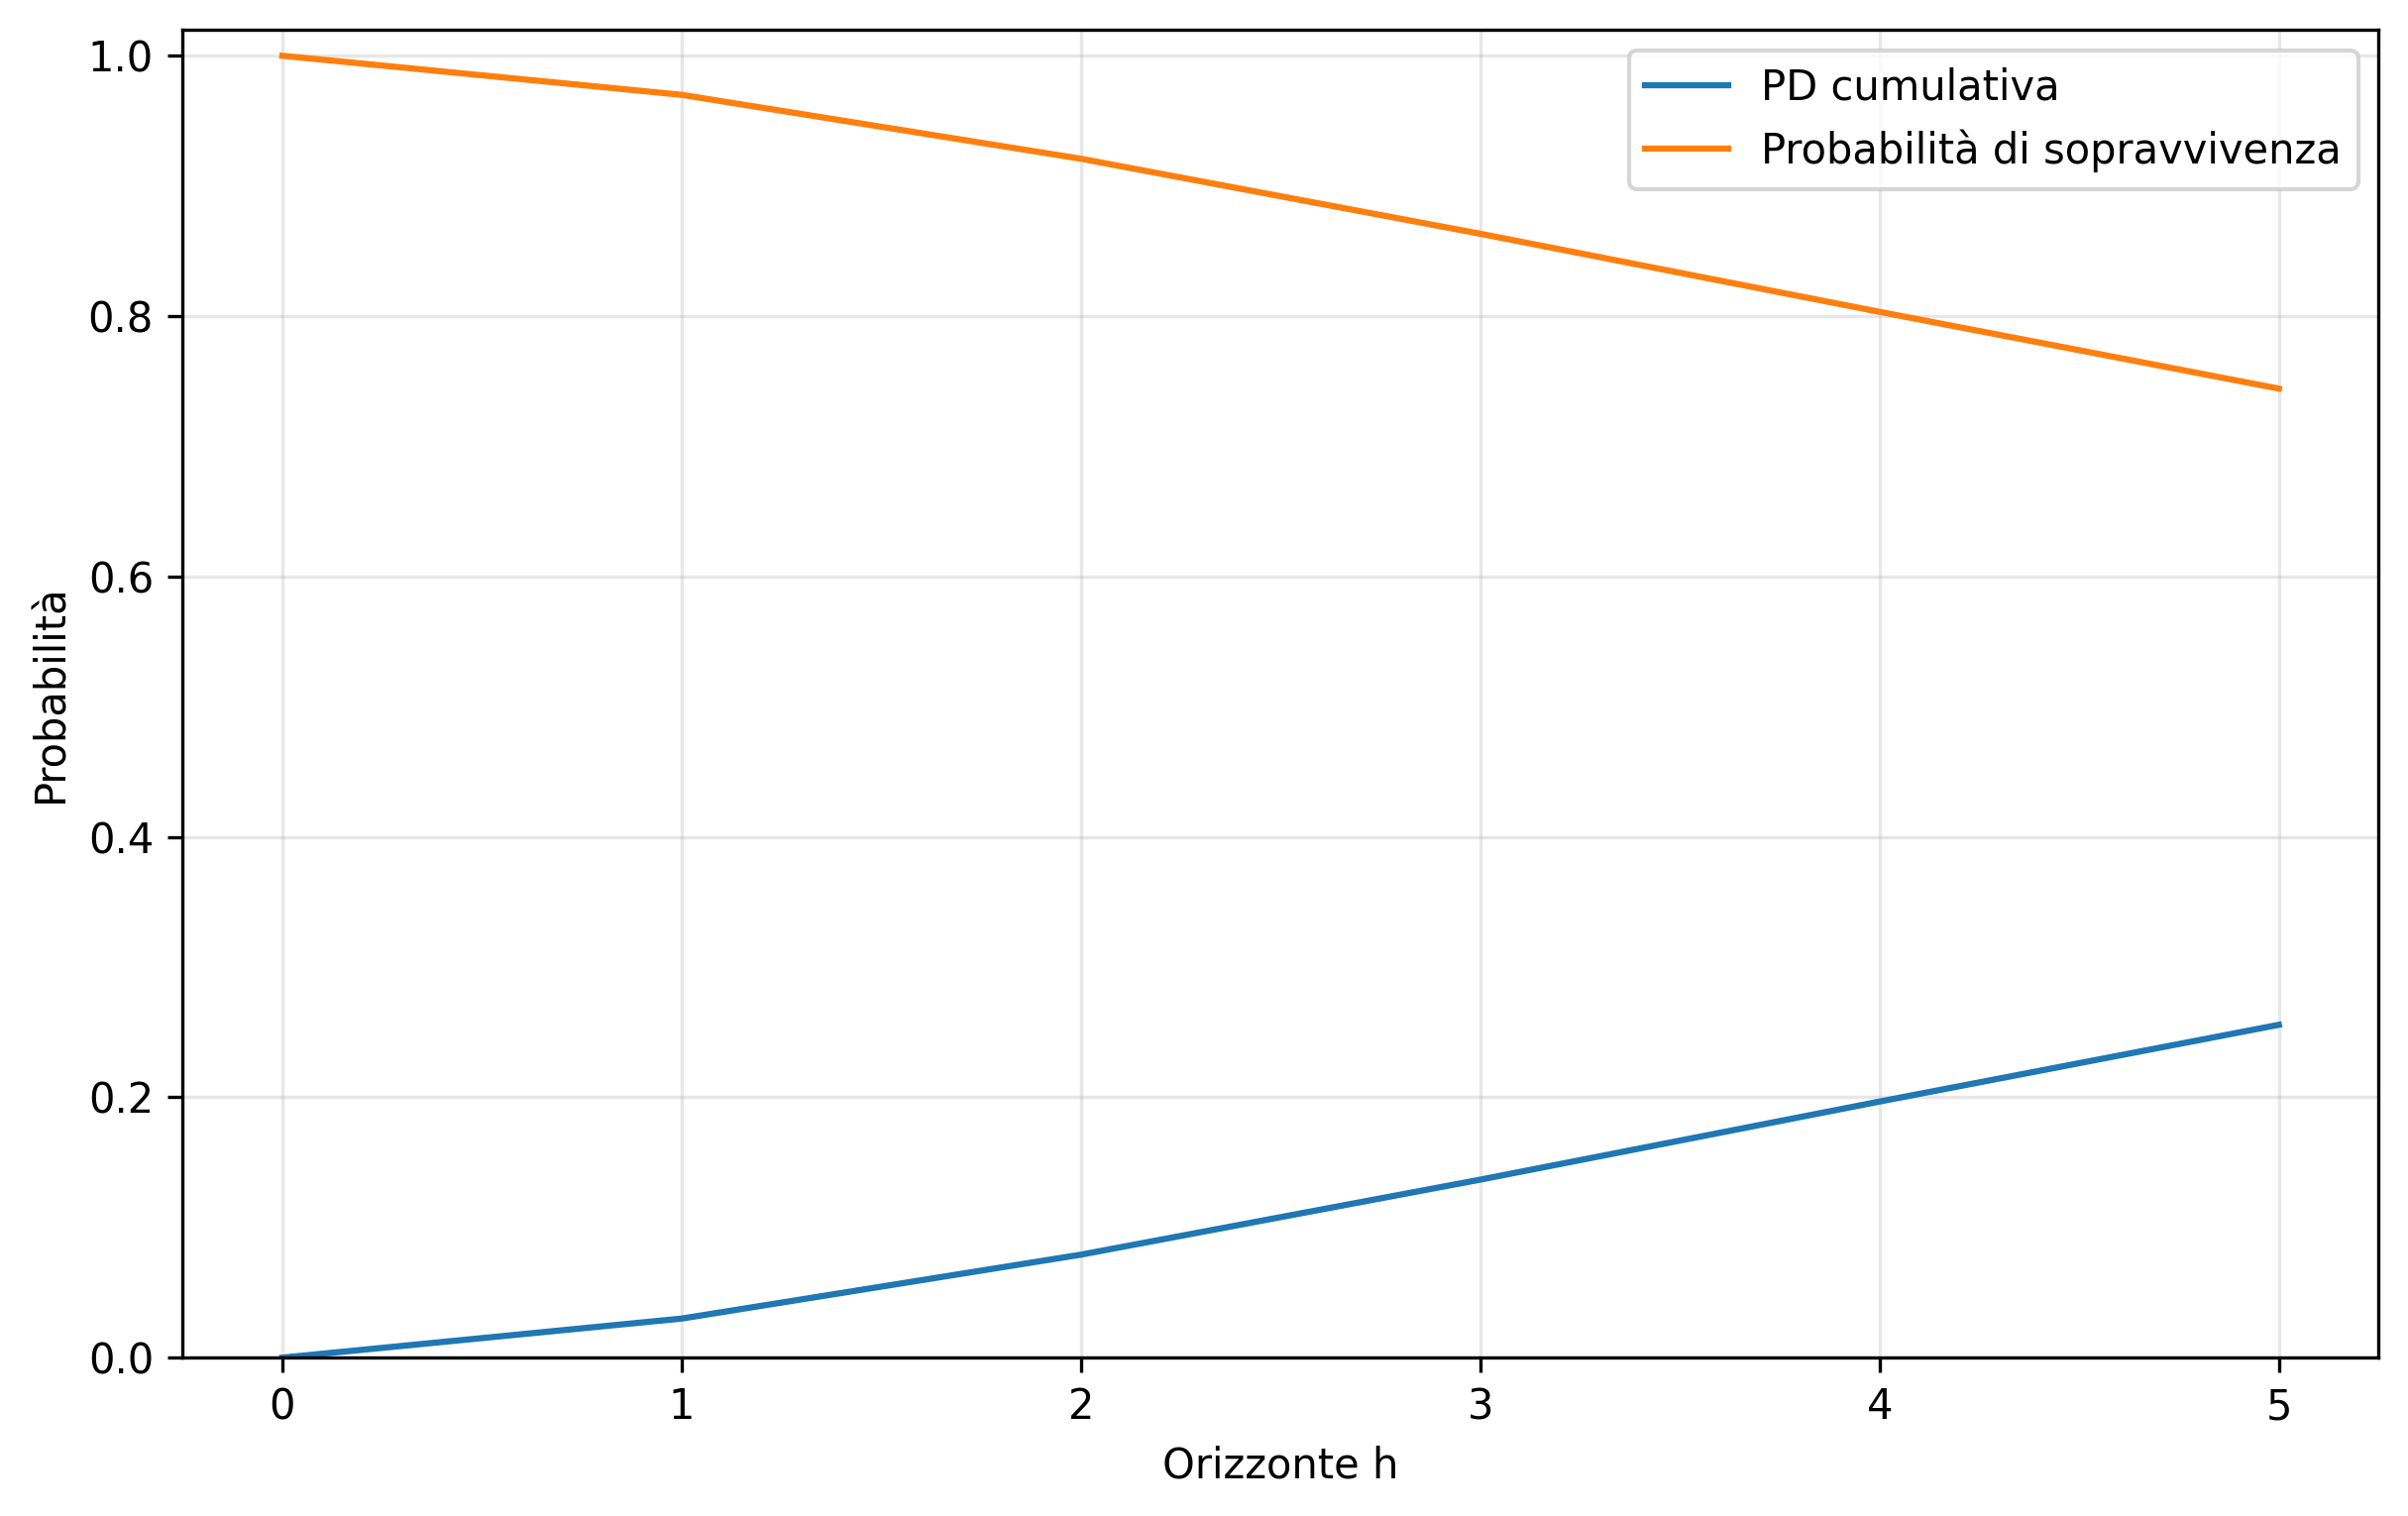
\includegraphics[height=6.2cm]{../graphics/Cap09_term_structure_default_esercizio.png}
\end{center}

\medskip

\begin{center}
{\small La PD cumulativa non decresce; la sopravvivenza \`{e} la sua
immagine speculare rispetto a $1$. La pendenza tra due date
consecutive \`{e} la probabilit\`{a} \textbf{marginale} di quel
periodo.}
\end{center}

%TCIMACRO{\TeXButton{Transition: Box Out}{\transboxout}}%
%BeginExpansion
\transboxout%
%EndExpansion
%TCIMACRO{\TeXButton{EndFrame}{\end{frame}}}%
%BeginExpansion
\end{frame}%
%EndExpansion

%***********************************************************

%***********************************************************

\section{Dalle probabilit\`{a} alle conseguenze economiche}

\subsection{PD, LGD, EAD}

%TCIMACRO{\TeXButton{BeginFrame}{\begin{frame}}}%
%BeginExpansion
\begin{frame}%
%EndExpansion

\QTR{frametitle}{PD, LGD, EAD e recovery rate}

%TCIMACRO{\TeXButton{Transparency}{\setbeamercovered{transparent=20}}}%
%BeginExpansion
\setbeamercovered{transparent=20}%
%EndExpansion

Il modello elementare della perdita da default combina tre parametri:

\medskip

\begin{stepitemize}
\item $\mathrm{PD}$ (\emph{probability of default}): nel modello
markoviano \`{e} determinata da matrice, stato iniziale e orizzonte,
\[
\mathrm{PD}_{i}^{\mathrm{cum}}(h)=(P^h)_{iD}.
\]
Non \`{e} una propriet\`{a} assoluta dell'emittente.

\item $\mathrm{EAD}$ (\emph{exposure at default}): ammontare
\textbf{monetario} esposto al momento del default; non coincide
necessariamente con il nominale iniziale.

\item $\mathrm{LGD}$ (\emph{loss given default}): quota
dell'esposizione perduta, $0\leq\mathrm{LGD}\leq 1$; complementare del
\emph{recovery rate}, $R=1-\mathrm{LGD}$.
\end{stepitemize}

\medskip

\begin{center}
{\small Probabilit\`{a} dell'evento, severit\`{a}, esposizione: solo
la loro \textbf{combinazione} produce una quantit\`{a} monetaria.}
\end{center}

%TCIMACRO{\TeXButton{Transition: Box Out}{\transboxout}}%
%BeginExpansion
\transboxout%
%EndExpansion
%TCIMACRO{\TeXButton{EndFrame}{\end{frame}}}%
%BeginExpansion
\end{frame}%
%EndExpansion

%***********************************************************
\subsection{Perdita da default e da migrazione}

%TCIMACRO{\TeXButton{BeginFrame}{\begin{frame}}}%
%BeginExpansion
\begin{frame}%
%EndExpansion

\QTR{frametitle}{Perdita da default e perdita da migrazione}

%TCIMACRO{\TeXButton{Transparency}{\setbeamercovered{transparent=20}}}%
%BeginExpansion
\setbeamercovered{transparent=20}%
%EndExpansion

Con $\mathrm{EAD}_h$ e $\mathrm{LGD}_h$ deterministici, la perdita da
\textbf{default} entro $h$ \`{e}
\[
L_h^{D}
=
\mathrm{EAD}_h\,
\mathrm{LGD}_h\,
\mathbf{1}_{\{\tau_D\leq h\}}.
\]

\medskip

\begin{stepitemize}
\item Ma il valore pu\`{o} ridursi anche \textbf{senza} default:
\[
\text{downgrade}
\longrightarrow
\text{aumento del credit spread}
\longrightarrow
\text{riduzione del valore}.
\]

\item A ogni stato futuro $j\in\mathcal{I}$ associamo un valore
$V_j(h)$: per un'obbligazione, i flussi residui attualizzati con
fattori di sconto coerenti con il rating $j$.

\item Fissato un riferimento $V^{\mathrm{ref}}(h)$, la perdita
associata allo stato $j$ \`{e}
\[
\ell(j,h)
=
V^{\mathrm{ref}}(h)-V_j(h).
\]
\end{stepitemize}

%TCIMACRO{\TeXButton{Transition: Box Out}{\transboxout}}%
%BeginExpansion
\transboxout%
%EndExpansion
%TCIMACRO{\TeXButton{EndFrame}{\end{frame}}}%
%BeginExpansion
\end{frame}%
%EndExpansion

%***********************************************************
\subsection{Default-only (DO) e migration-based}

%TCIMACRO{\TeXButton{BeginFrame}{\begin{frame}}}%
%BeginExpansion
\begin{frame}%
%EndExpansion

\QTR{frametitle}{Modello default-only e modello migration-based}

%TCIMACRO{\TeXButton{Transparency}{\setbeamercovered{transparent=20}}}%
%BeginExpansion
\setbeamercovered{transparent=20}%
%EndExpansion

\[
\ell_j^{\mathrm{DO}}(h)
=
\begin{cases}
0, & j\neq D,\\[1mm]
\mathrm{EAD}_h\mathrm{LGD}_h, & j=D,
\end{cases}
\qquad
\ell_j^{\mathrm{MB}}(h)
=
V^{\mathrm{ref}}(h)-V_j(h).
\]

\medskip

\[
\begin{array}{lll}
\hline
& \text{default-only} & \text{migration-based}\\
\hline
\text{stati rilevanti} & \text{default e sopravvivenza} & \text{tutti
i rating futuri}\\
\text{perdite non-default} & \text{nulle} & \text{positive o negative}\\
\text{informazione usata} & (P^h)_{iD} & \text{intera riga $i$ di }P^h\\
\text{applicazione} & \text{perdita da default} & \text{rischio
mark-to-market}\\
\hline
\end{array}
\]

\medskip

\begin{stepitemize}
\item Le esposizioni $A$ e $B$ dell'apertura: stessa PD, downgrade
$0.15$ contro $0.02$.

\item Nel modello default-only sono \textbf{indistinguibili}; nel
modello migration-based producono distribuzioni di perdita diverse.
\end{stepitemize}

%TCIMACRO{\TeXButton{Transition: Box Out}{\transboxout}}%
%BeginExpansion
\transboxout%
%EndExpansion
%TCIMACRO{\TeXButton{EndFrame}{\end{frame}}}%
%BeginExpansion
\end{frame}%
%EndExpansion

%***********************************************************

\section{La distribuzione della perdita}

\subsection{La funzione di perdita}

%TCIMACRO{\TeXButton{BeginFrame}{\begin{frame}}}%
%BeginExpansion
\begin{frame}%
%EndExpansion

\QTR{frametitle}{Dallo stato futuro alla perdita}

%TCIMACRO{\TeXButton{Transparency}{\setbeamercovered{transparent=20}}}%
%BeginExpansion
\setbeamercovered{transparent=20}%
%EndExpansion

La perdita all'orizzonte $h$ \`{e} una \textbf{variabile casuale},
funzione dello stato futuro della catena:
\[
L_h
=
\ell(X_h,h),
\qquad
\ell(j,h)=V^{\mathrm{ref}}(h)-V_j(h).
\]

\medskip

\begin{stepitemize}
\item L'aleatoriet\`{a} di $L_h$ deriva interamente da quella di
$X_h$: la catena fornisce le \textbf{probabilit\`{a}}, il modello
economico fornisce i \textbf{valori}.

\item Convenzione sul segno: valori \emph{positivi} di $L_h$
rappresentano perdite, valori \emph{negativi} guadagni. Tutte le
misure di rischio della lezione adottano questa convenzione.

\item Condizionatamente a $X_0=i$, la distribuzione di $L_h$ si
ottiene trasferendo la riga $i$ di $P^h$ sui valori $\ell(j,h)$.
\end{stepitemize}

%TCIMACRO{\TeXButton{Transition: Box Out}{\transboxout}}%
%BeginExpansion
\transboxout%
%EndExpansion
%TCIMACRO{\TeXButton{EndFrame}{\end{frame}}}%
%BeginExpansion
\end{frame}%
%EndExpansion

%***********************************************************
\subsection{Il caso guida}

%TCIMACRO{\TeXButton{BeginFrame}{\begin{frame}}}%
%BeginExpansion
\begin{frame}%
%EndExpansion

\QTR{frametitle}{Caso guida: tabella stato--probabilit\`{a}--valore--perdita}

%TCIMACRO{\TeXButton{Transparency}{\setbeamercovered{transparent=20}}}%
%BeginExpansion
\setbeamercovered{transparent=20}%
%EndExpansion

Matrice di migrazione del Capitolo~8, emittente in classe intermedia
($X_0=2$), orizzonte $h=1$, $V^{\mathrm{ref}}(1)=100$:
\[
P_R
=
\begin{pmatrix}
0.80 & 0.18 & 0.02 & 0.00\\
0.08 & 0.75 & 0.14 & 0.03\\
0.02 & 0.18 & 0.65 & 0.15\\
0.00 & 0.00 & 0.00 & 1.00
\end{pmatrix},
\qquad
\begin{array}{l}
V_1(1)=103,\\
V_2(1)=100,\\
V_3(1)=92,\\
V_D(1)=40.
\end{array}
\]

\medskip

\[
\begin{array}{lcccc}
\hline
\text{rating futuro} & \text{probabilit\`{a}} & V_j(1) & \ell_j(1) &
\text{prob. cumulata}\\
\hline
1 & 0.08 & 103 & -3 & 0.08\\
2 & 0.75 & 100 & 0 & 0.83\\
3 & 0.14 & 92 & 8 & 0.97\\
D & 0.03 & 40 & 60 & 1.00\\
\hline
\end{array}
\]

\medskip

\begin{center}
{\small Le probabilit\`{a} derivano dalla \textbf{catena}; valori e
perdite dal \textbf{modello economico}. Questa tabella sar\`{a} il
riferimento per EL, VaR e CVaR.}
\end{center}

%TCIMACRO{\TeXButton{Transition: Box Out}{\transboxout}}%
%BeginExpansion
\transboxout%
%EndExpansion
%TCIMACRO{\TeXButton{EndFrame}{\end{frame}}}%
%BeginExpansion
\end{frame}%
%EndExpansion

%***********************************************************
\subsection{Esercizio A}

%TCIMACRO{\TeXButton{BeginFrame}{\begin{frame}}}%
%BeginExpansion
\begin{frame}%
%EndExpansion

\QTR{frametitle}{Esercizio A: la distribuzione della perdita}

Emittente con $X_0=2$; distribuzione del rating a un anno, valore di
riferimento e valori per stato:
\[
\begin{array}{c|cccc}
j & 1 & 2 & 3 & D\\
\hline
\Prob(X_1=j\mid X_0=2) & 0.05 & 0.78 & 0.14 & 0.03\\
V_j(1) & 104 & 100 & 90 & 45
\end{array}
\qquad
V^{\mathrm{ref}}(1)=100.
\]

\medskip

Posto $L_1=\ell(X_1,1)$ con $\ell(j,1)=V^{\mathrm{ref}}(1)-V_j(1)$:

\begin{enumerate}
\item[1.] Determinare la perdita associata a ciascun rating futuro.

\item[2.] Costruire la funzione di massa di $L_1$.

\item[3.] Determinare la funzione di ripartizione $F_{L_1}$.

\item[4.] Calcolare la perdita attesa e interpretare i contributi dei
diversi stati.
\end{enumerate}

\medskip

\begin{center}
{\small Lavoro individuale o a coppie: circa 10 minuti. Seguir\`{a} la
discussione.}
\end{center}

%TCIMACRO{\TeXButton{Transition: Box Out}{\transboxout}}%
%BeginExpansion
\transboxout%
%EndExpansion
%TCIMACRO{\TeXButton{EndFrame}{\end{frame}}}%
%BeginExpansion
\end{frame}%
%EndExpansion

%***********************************************************
\subsection{Esercizio A: discussione}

%TCIMACRO{\TeXButton{BeginFrame}{\begin{frame}}}%
%BeginExpansion
\begin{frame}%
%EndExpansion

\QTR{frametitle}{Esercizio A: discussione}

%TCIMACRO{\TeXButton{Transparency}{\setbeamercovered{transparent=20}}}%
%BeginExpansion
\setbeamercovered{transparent=20}%
%EndExpansion

\begin{center}
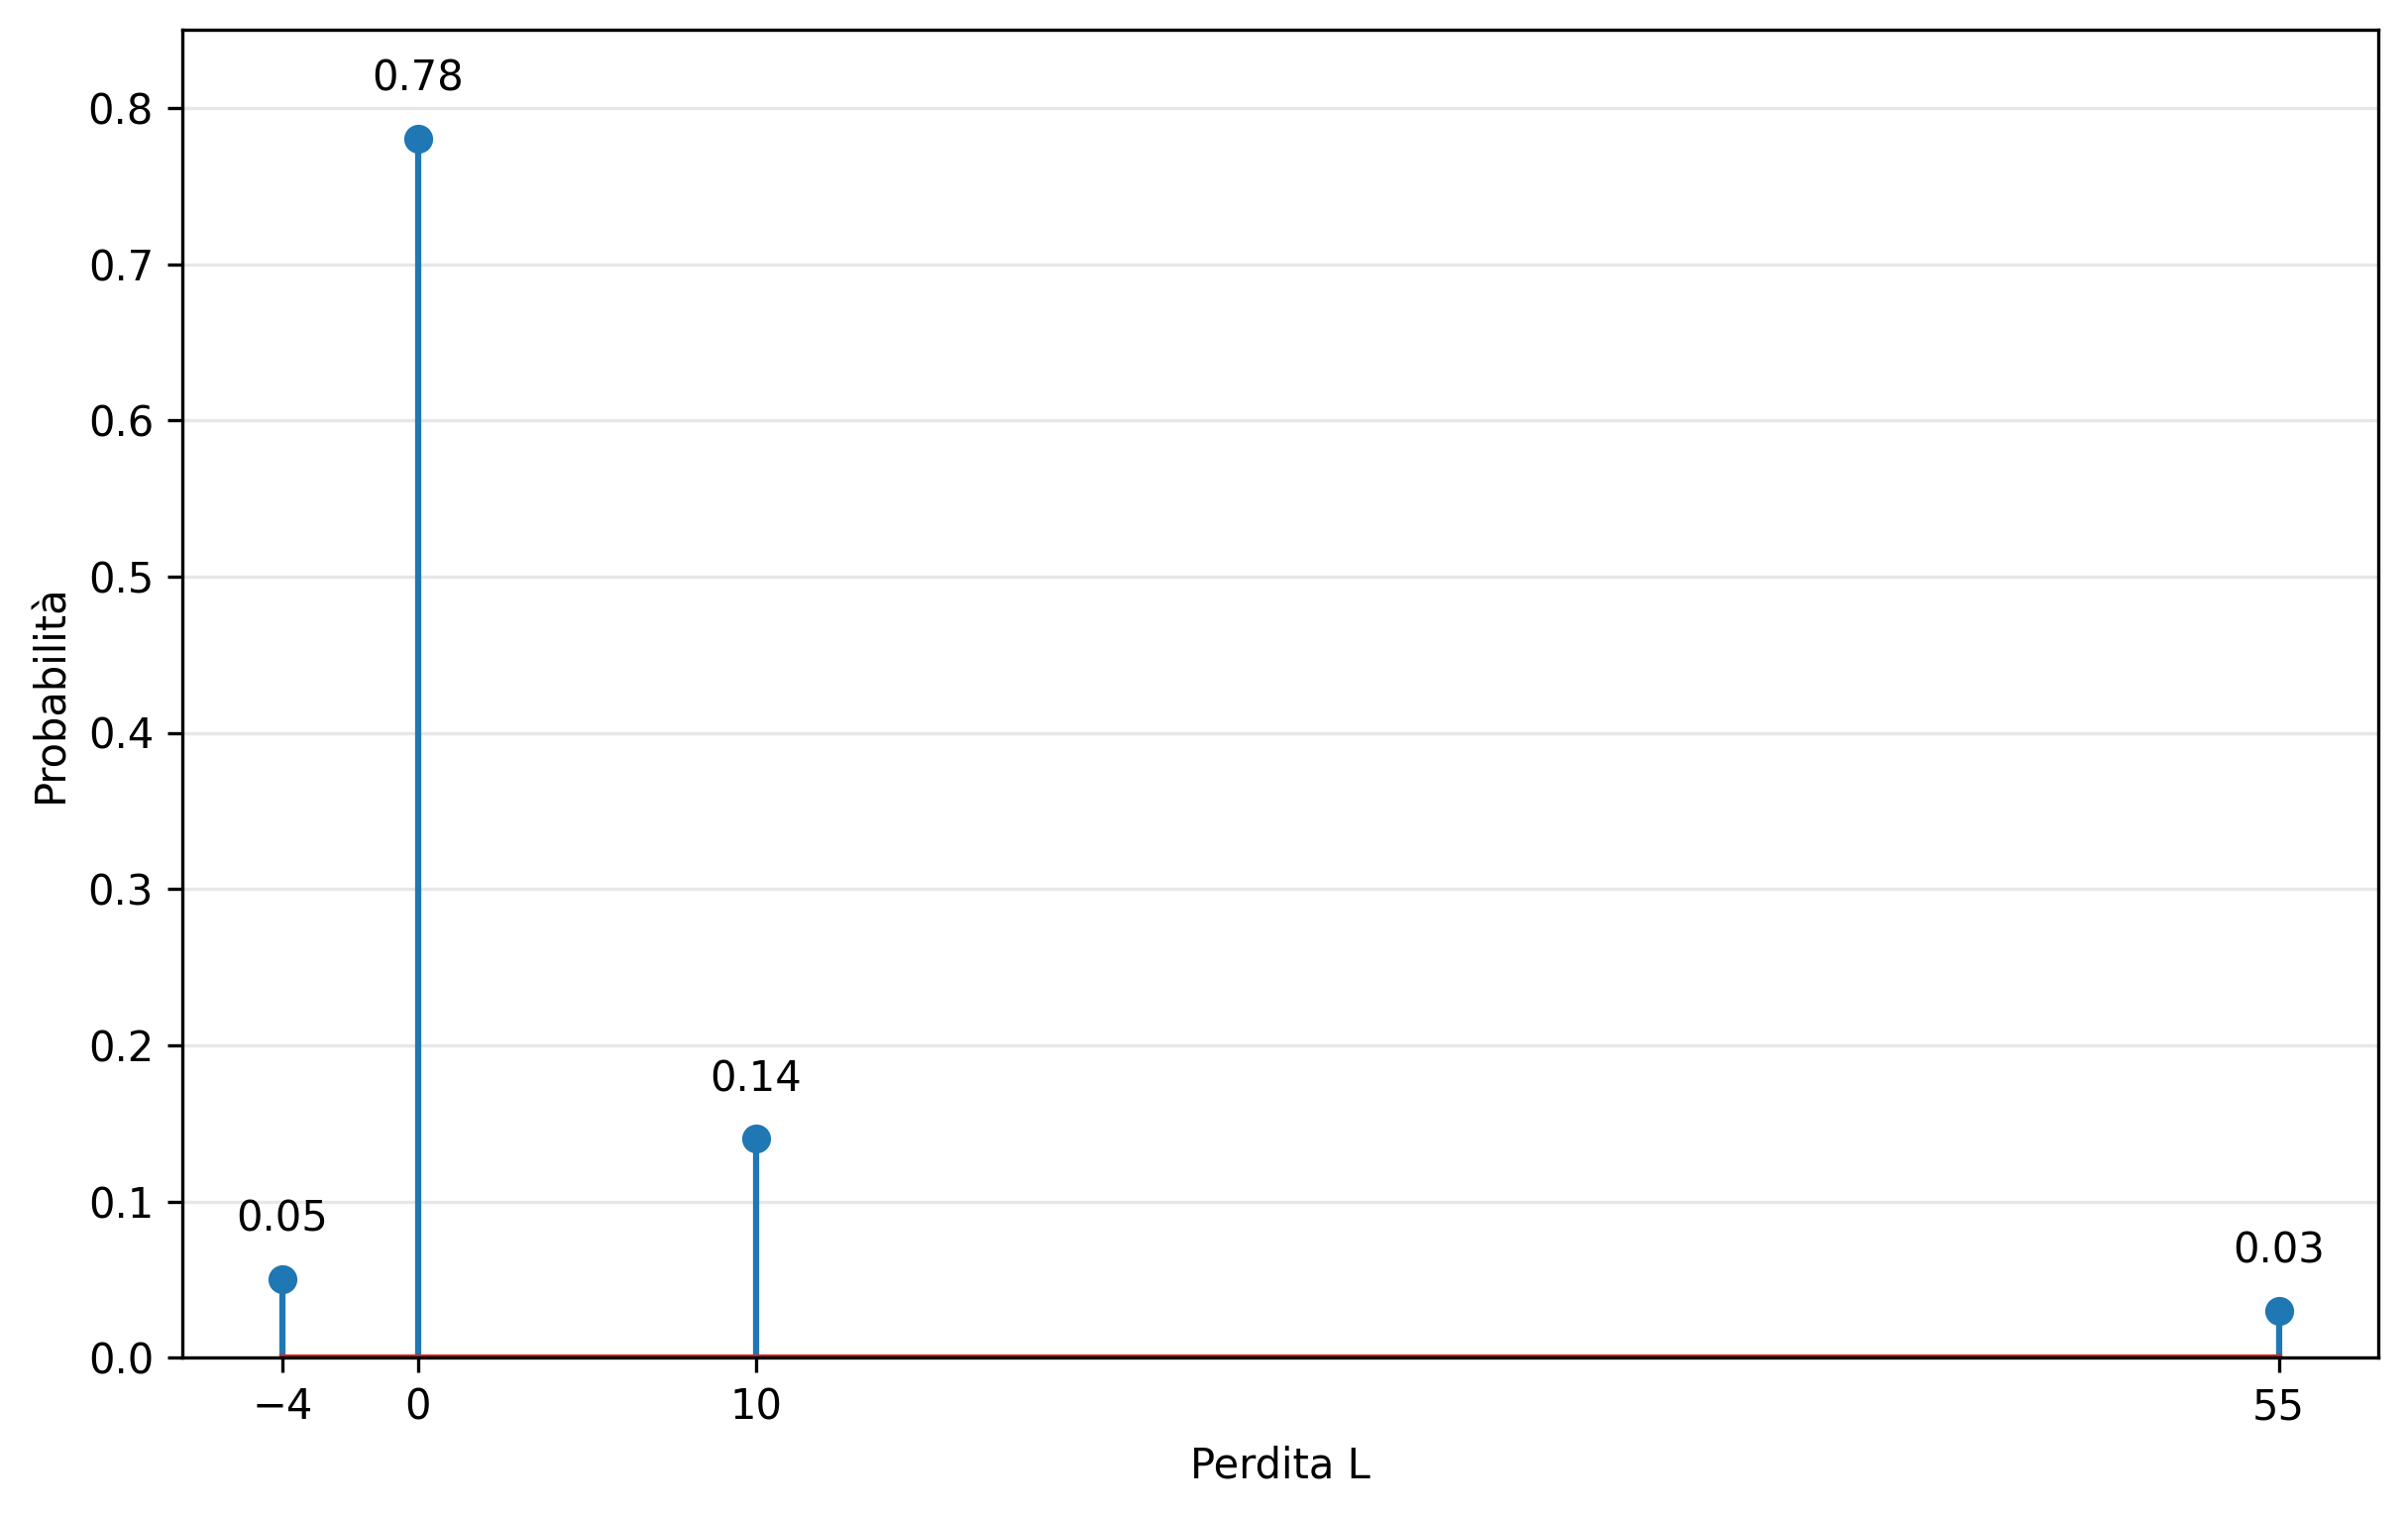
\includegraphics[height=4.6cm]{../graphics/Cap09_distribuzione_perdita_esercizio.png}
\end{center}

\medskip

\begin{stepitemize}
\item Perch\'{e} la massa dominante \`{e} in $L_1=0$? Che cosa dice
sulla natura del rischio di credito?

\item La perdita $-4$ \`{e} un \textbf{guadagno}: quale evento la
genera, e perch\'{e} la convenzione sul segno la rappresenta cos\`{\i}?

\item Il default: perdita elevata ($55$), probabilit\`{a} piccola
($0.03$). \`{E} questa asimmetria a rendere insufficiente la sola
perdita attesa.
\end{stepitemize}

%TCIMACRO{\TeXButton{Transition: Box Out}{\transboxout}}%
%BeginExpansion
\transboxout%
%EndExpansion
%TCIMACRO{\TeXButton{EndFrame}{\end{frame}}}%
%BeginExpansion
\end{frame}%
%EndExpansion

%***********************************************************

%***********************************************************

\section{Perdita attesa e quantili}

\subsection{Expected Loss}

%TCIMACRO{\TeXButton{BeginFrame}{\begin{frame}}}%
%BeginExpansion
\begin{frame}%
%EndExpansion

\QTR{frametitle}{Expected Loss}

%TCIMACRO{\TeXButton{Transparency}{\setbeamercovered{transparent=20}}}%
%BeginExpansion
\setbeamercovered{transparent=20}%
%EndExpansion

Condizionatamente allo stato iniziale $X_0=i$, la \textbf{perdita
attesa} all'orizzonte $h$ \`{e}
\[
\mathrm{EL}_i(h)
=
\E[L_h\mid X_0=i]
=
\sum_{j\in\mathcal{I}}
\ell(j,h)(P^h)_{ij}.
\]

\medskip

\begin{stepitemize}
\item $P^h$ fornisce i pesi probabilistici, $\ell(j,h)$ le perdite
monetarie: la formula combina i due modelli.

\item Nel modello default-only la formula si riduce alla relazione
tradizionale
\[
\mathrm{EL}_i(h)
=
\mathrm{PD}_{i}^{\mathrm{cum}}(h)\,
\mathrm{LGD}_h\,
\mathrm{EAD}_h.
\]

\item Sul caso guida: $\mathrm{EL}_2(1)=(-3)(0.08)+0(0.75)
+8(0.14)+60(0.03)=2.68$.

\item La EL \`{e} un \textbf{costo atteso}, non una misura di rischio:
due distribuzioni con la stessa media possono avere dispersioni e code
molto diverse. Il rischio vive nella coda.
\end{stepitemize}

%TCIMACRO{\TeXButton{Transition: Box Out}{\transboxout}}%
%BeginExpansion
\transboxout%
%EndExpansion
%TCIMACRO{\TeXButton{EndFrame}{\end{frame}}}%
%BeginExpansion
\end{frame}%
%EndExpansion

%***********************************************************
\subsection{Quantili}

%TCIMACRO{\TeXButton{BeginFrame}{\begin{frame}}}%
%BeginExpansion
\begin{frame}%
%EndExpansion

\QTR{frametitle}{Quantili di distribuzioni discrete}

%TCIMACRO{\TeXButton{Transparency}{\setbeamercovered{transparent=20}}}%
%BeginExpansion
\setbeamercovered{transparent=20}%
%EndExpansion

Per $\alpha\in(0,1)$, il \textbf{quantile} di livello $\alpha$ della
perdita $L$ \`{e}
\[
q_{\alpha}(L)
=
\inf
\left\{
\ell\in\R:
F_L(\ell)\geq\alpha
\right\}.
\]

\medskip

\begin{stepitemize}
\item Il pi\`{u} piccolo valore monetario per cui la probabilit\`{a}
cumulata raggiunge \emph{almeno} $\alpha$.

\item Vale $\Prob(L\leq q_{\alpha}(L))\geq\alpha$, \textbf{non}
necessariamente con uguaglianza: nel caso discreto $\alpha$ pu\`{o}
cadere dentro un salto,
\[
F_L\left(q_{\alpha}(L)^{-}\right)
\leq
\alpha
\leq
F_L\left(q_{\alpha}(L)\right).
\]

\item Il quantile \textbf{appartiene al supporto}: nessuna
interpolazione tra valori discreti.

\item Ricetta operativa: ordinare le perdite (non i codici degli
stati!), cumulare le probabilit\`{a}, selezionare la prima perdita che
raggiunge $\alpha$.
\end{stepitemize}

%TCIMACRO{\TeXButton{Transition: Box Out}{\transboxout}}%
%BeginExpansion
\transboxout%
%EndExpansion
%TCIMACRO{\TeXButton{EndFrame}{\end{frame}}}%
%BeginExpansion
\end{frame}%
%EndExpansion

%***********************************************************
\subsection{Lettura grafica}

%TCIMACRO{\TeXButton{BeginFrame}{\begin{frame}}}%
%BeginExpansion
\begin{frame}%
%EndExpansion

\QTR{frametitle}{Il quantile sulla funzione di ripartizione}

Caso guida ($X_0=2$, $h=1$), livello $\alpha=0.95$:
\[
F_{L_1\mid 2}(0)=0.83<0.95,
\qquad
F_{L_1\mid 2}(8)=0.97\geq0.95
\quad\Longrightarrow\quad
q_{0.95}(L_1\mid X_0=2)=8.
\]

\medskip

\begin{center}
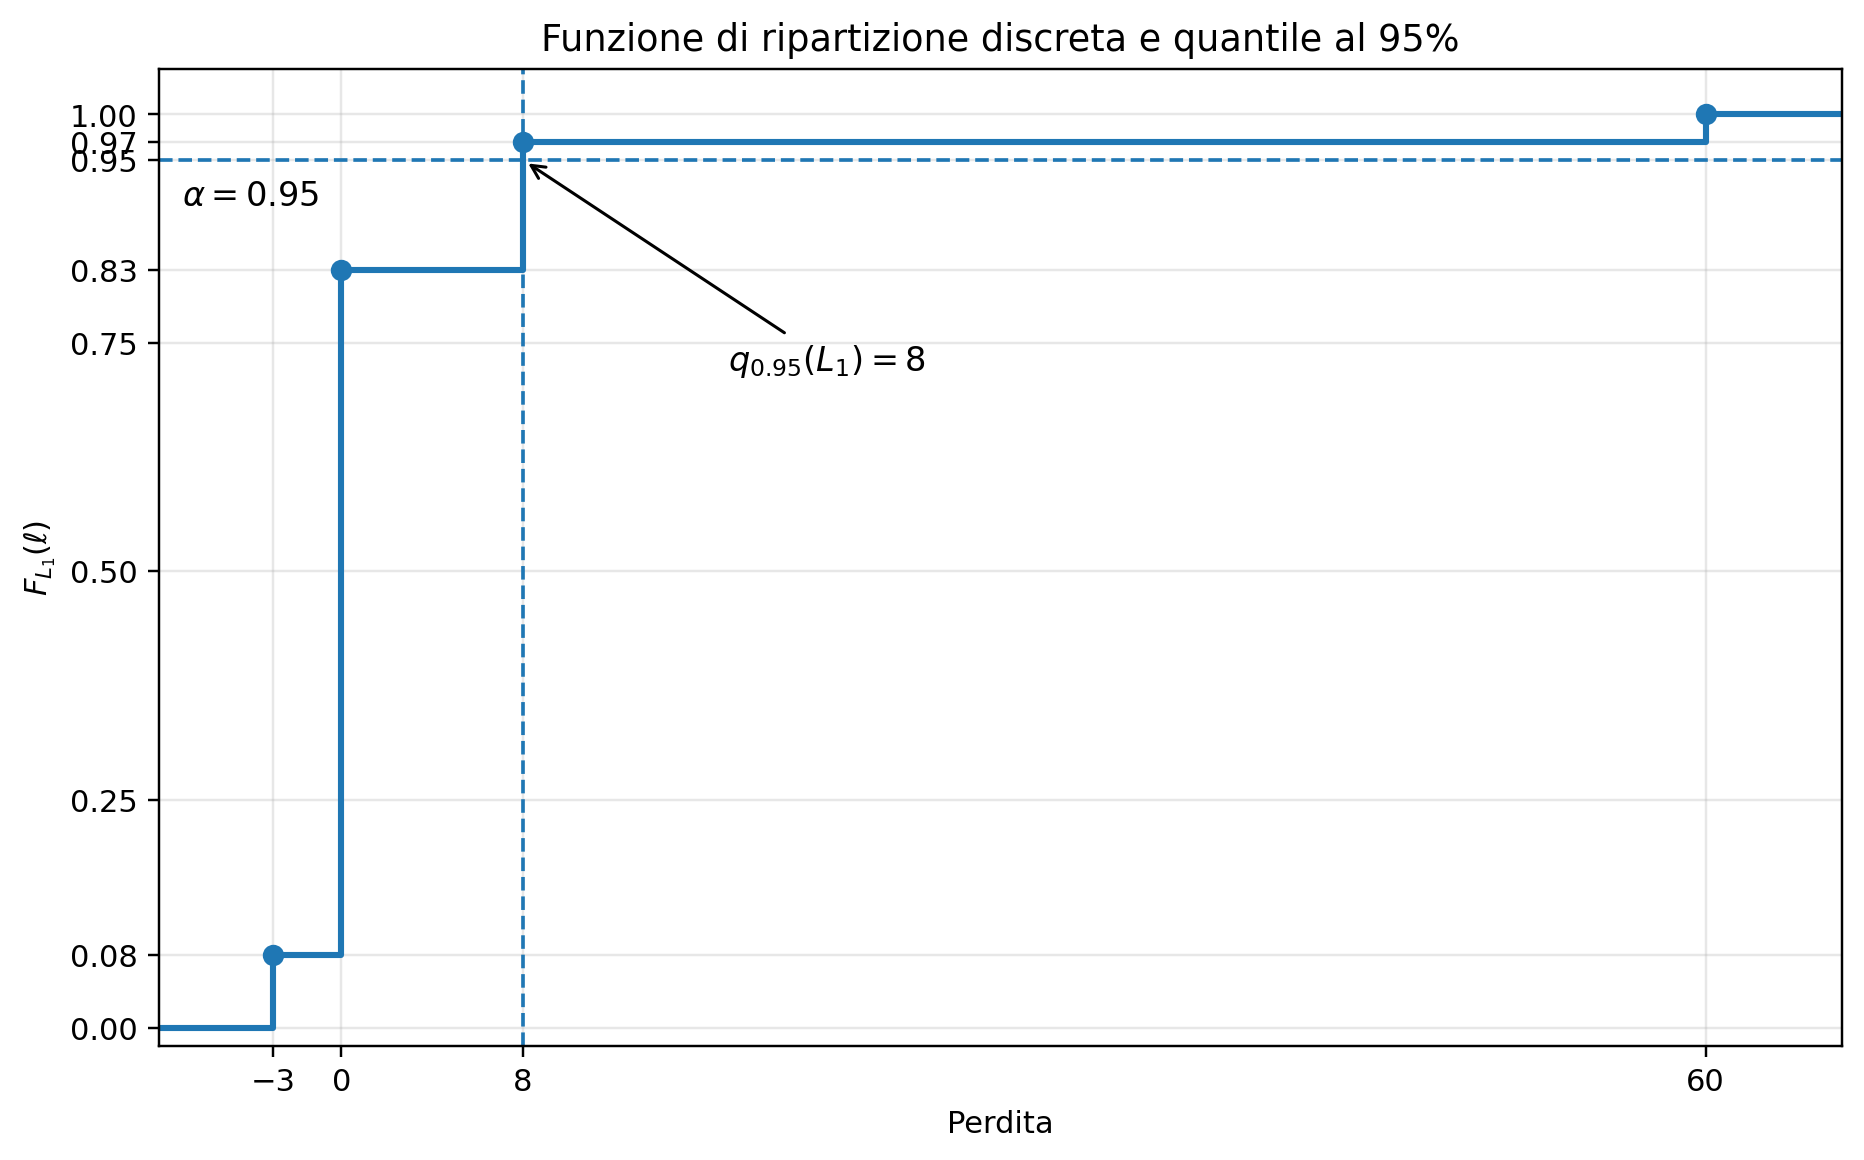
\includegraphics[height=4.9cm]{../graphics/Cap09_funzione_ripartizione_quantile.png}
\end{center}

\medskip

\begin{center}
{\small Il livello $0.95$ cade \emph{dentro} il salto di ampiezza
$0.14$ in $\ell=8$. Il quantile resta costante per interi intervalli
di $\alpha$ e cambia bruscamente oltre una cumulata: per
$\alpha=0.97$ vale ancora $8$, appena oltre vale $60$.}
\end{center}

%TCIMACRO{\TeXButton{Transition: Box Out}{\transboxout}}%
%BeginExpansion
\transboxout%
%EndExpansion
%TCIMACRO{\TeXButton{EndFrame}{\end{frame}}}%
%BeginExpansion
\end{frame}%
%EndExpansion

%***********************************************************

\section{Value at Risk creditizio}

\subsection{Definizione}

%TCIMACRO{\TeXButton{BeginFrame}{\begin{frame}}}%
%BeginExpansion
\begin{frame}%
%EndExpansion

\QTR{frametitle}{Value at Risk}

%TCIMACRO{\TeXButton{Transparency}{\setbeamercovered{transparent=20}}}%
%BeginExpansion
\setbeamercovered{transparent=20}%
%EndExpansion

Il Value at Risk \`{e} il quantile della perdita, interpretato come
\textbf{soglia monetaria di rischio}:
\[
\VaR_{\alpha}(L)
=
q_{\alpha}(L)
=
\inf
\left\{
\ell\in\R:
F_L(\ell)\geq\alpha
\right\}.
\]

\medskip

\begin{stepitemize}
\item Nel contesto creditizio, condizionatamente allo stato iniziale:
\[
\VaR_{\alpha,i}(h)
=
q_{\alpha}(L_h\mid X_0=i).
\]

\item Sul caso guida:
\[
\VaR_{0.95,2}(1)=8:
\]
la pi\`{u} piccola soglia per cui la probabilit\`{a} cumulata delle
perdite raggiunge almeno il $95\%$.

\item In una distribuzione discreta $\Prob(L\leq\VaR_{\alpha}(L))$
pu\`{o} essere \emph{strettamente} maggiore di $\alpha$: qui vale
$0.97$.
\end{stepitemize}

%TCIMACRO{\TeXButton{Transition: Box Out}{\transboxout}}%
%BeginExpansion
\transboxout%
%EndExpansion
%TCIMACRO{\TeXButton{EndFrame}{\end{frame}}}%
%BeginExpansion
\end{frame}%
%EndExpansion

%***********************************************************
\subsection{Orizzonte e confidenza}

%TCIMACRO{\TeXButton{BeginFrame}{\begin{frame}}}%
%BeginExpansion
\begin{frame}%
%EndExpansion

\QTR{frametitle}{Orizzonte e livello di confidenza}

%TCIMACRO{\TeXButton{Transparency}{\setbeamercovered{transparent=20}}}%
%BeginExpansion
\setbeamercovered{transparent=20}%
%EndExpansion

Un valore di VaR non \`{e} interpretabile senza specificare:

\begin{stepitemize}
\item l'orizzonte temporale $h$;

\item il livello di confidenza $\alpha$;

\item l'unit\`{a} monetaria della perdita;

\item la distribuzione di $L_h$ e il modello che la genera.
\end{stepitemize}

\medskip

Incompleta: \emph{``il VaR \`{e} pari a 8''.}

\smallskip

Corretta: \emph{``il VaR al $95\%$ della perdita a un anno,
condizionatamente al rating iniziale $i=2$, \`{e} pari a $8$
unit\`{a} monetarie nel modello di transizione considerato''.}

\medskip

\begin{center}
{\small $\alpha$ e $h$ sono \textbf{convenzioni della misura}, non
propriet\`{a} dell'esposizione: cambiando orizzonte cambiano sia le
probabilit\`{a}, tramite $P^h$, sia i valori, tramite $\ell(j,h)$.}
\end{center}

%TCIMACRO{\TeXButton{Transition: Box Out}{\transboxout}}%
%BeginExpansion
\transboxout%
%EndExpansion
%TCIMACRO{\TeXButton{EndFrame}{\end{frame}}}%
%BeginExpansion
\end{frame}%
%EndExpansion

%***********************************************************

%***********************************************************

\section{Conditional Value at Risk}

\subsection{Limiti del VaR}

%TCIMACRO{\TeXButton{BeginFrame}{\begin{frame}}}%
%BeginExpansion
\begin{frame}%
%EndExpansion

\QTR{frametitle}{Che cosa il VaR non vede}

%TCIMACRO{\TeXButton{Transparency}{\setbeamercovered{transparent=20}}}%
%BeginExpansion
\setbeamercovered{transparent=20}%
%EndExpansion

Posto $v=\VaR_{\alpha}(L)$:

\medskip

\begin{stepitemize}
\item \textbf{Il VaR non \`{e} la massima perdita possibile.} Da
$\Prob(L\leq v)\geq\alpha$ segue $\Prob(L>v)\leq 1-\alpha$: una quota
fino a $1-\alpha$ della distribuzione sta \emph{oltre} la soglia.

\item \textbf{Il VaR non descrive la severit\`{a} oltre la soglia.}
Se la coda estrema diventa pi\`{u} severa ma il quantile non cambia,
il VaR resta invariato: due distribuzioni possono avere lo stesso VaR
e scenari estremi molto diversi.

\item \textbf{Il VaR pu\`{o} non essere subadditivo}: aggregando due
posizioni, la misura del portafoglio pu\`{o} superare la somma delle
misure individuali.
\end{stepitemize}

\medskip

\begin{center}
{\small Il secondo limite \`{e} quello che ora tocchiamo con mano:
lavoriamo su due distribuzioni costruite apposta.}
\end{center}

%TCIMACRO{\TeXButton{Transition: Box Out}{\transboxout}}%
%BeginExpansion
\transboxout%
%EndExpansion
%TCIMACRO{\TeXButton{EndFrame}{\end{frame}}}%
%BeginExpansion
\end{frame}%
%EndExpansion

%***********************************************************
\subsection{Esercizio B}

%TCIMACRO{\TeXButton{BeginFrame}{\begin{frame}}}%
%BeginExpansion
\begin{frame}%
%EndExpansion

\QTR{frametitle}{Esercizio B: stesso VaR, code diverse}

Due distribuzioni discrete di perdita:
\[
\begin{array}{c|cccc}
\lambda & 0 & 10 & 20 & 100\\
\hline
\Prob(L_A=\lambda) & 0.90 & 0.05 & 0.04 & 0.01\\
\Prob(L_B=\lambda) & 0.90 & 0.05 & 0.01 & 0.04
\end{array}
\]

\medskip

\begin{enumerate}
\item[1.] Costruire le funzioni di ripartizione di $L_A$ e $L_B$.

\item[2.] Calcolare il VaR al livello del $95\%$ per entrambe.

\item[3.] Confrontare le due code oltre la soglia: quale posizione \`{e}
pi\`{u} rischiosa? Il VaR rileva questa differenza?
\end{enumerate}

\medskip

\begin{center}
{\small Lavoro individuale o a coppie: circa 10 minuti. Seguir\`{a} la
discussione.}
\end{center}

%TCIMACRO{\TeXButton{Transition: Box Out}{\transboxout}}%
%BeginExpansion
\transboxout%
%EndExpansion
%TCIMACRO{\TeXButton{EndFrame}{\end{frame}}}%
%BeginExpansion
\end{frame}%
%EndExpansion

%***********************************************************
\subsection{Esercizio B: discussione}

%TCIMACRO{\TeXButton{BeginFrame}{\begin{frame}}}%
%BeginExpansion
\begin{frame}%
%EndExpansion

\QTR{frametitle}{Esercizio B: discussione}

%TCIMACRO{\TeXButton{Transparency}{\setbeamercovered{transparent=20}}}%
%BeginExpansion
\setbeamercovered{transparent=20}%
%EndExpansion

Raccogliamo e verifichiamo i risultati.

\medskip

\begin{stepitemize}
\item Le cumulate coincidono fino a $\lambda=10$: in particolare
$F_{L_A}(10)=F_{L_B}(10)=0.95$. Pertanto
\[
\VaR_{0.95}(L_A)
=
\VaR_{0.95}(L_B)
=
10.
\]

\item Ma oltre la soglia le code sono molto diverse: $L_A$ colloca in
$100$ una probabilit\`{a} $0.01$, $L_B$ una probabilit\`{a} $0.04$.

\item Un risk manager preferirebbe la posizione $A$; il VaR le
dichiara \textbf{equivalenti}.
\end{stepitemize}

\medskip

Domanda di interpretazione:

\begin{stepitemize}
\item Quale caratteristica della distribuzione dovrebbe misurare un
indicatore capace di distinguere $A$ da $B$?
\end{stepitemize}

%TCIMACRO{\TeXButton{Transition: Box Out}{\transboxout}}%
%BeginExpansion
\transboxout%
%EndExpansion
%TCIMACRO{\TeXButton{EndFrame}{\end{frame}}}%
%BeginExpansion
\end{frame}%
%EndExpansion

%***********************************************************
\subsection{Definizione di CVaR}

%TCIMACRO{\TeXButton{BeginFrame}{\begin{frame}}}%
%BeginExpansion
\begin{frame}%
%EndExpansion

\QTR{frametitle}{Conditional Value at Risk}

%TCIMACRO{\TeXButton{Transparency}{\setbeamercovered{transparent=20}}}%
%BeginExpansion
\setbeamercovered{transparent=20}%
%EndExpansion

La risposta: mediare i quantili della coda peggiore.

\medskip

Per $\alpha\in(0,1)$, il \emph{Conditional Value at Risk} di livello
$\alpha$ \`{e}
\[
\CVaR_{\alpha}(L)
=
\frac{1}{1-\alpha}
\int_{\alpha}^{1}
q_u(L)\,du.
\]

\medskip

\begin{stepitemize}
\item La media dei quantili appartenenti alla frazione $1-\alpha$
pi\`{u} sfavorevole della distribuzione: dipende dal punto in cui
inizia la coda \emph{e} dall'ampiezza delle perdite che la
costituiscono.

\item Convenzione del corso:
$\operatorname{ES}_{\alpha}(L)=\CVaR_{\alpha}(L)$ --- Expected
Shortfall e CVaR denominano la stessa misura.

\item Nel contesto creditizio:
$\CVaR_{\alpha,i}(h)=\CVaR_{\alpha}(L_h\mid X_0=i)$.
\end{stepitemize}

%TCIMACRO{\TeXButton{Transition: Box Out}{\transboxout}}%
%BeginExpansion
\transboxout%
%EndExpansion
%TCIMACRO{\TeXButton{EndFrame}{\end{frame}}}%
%BeginExpansion
\end{frame}%
%EndExpansion

%***********************************************************
\subsection{Massa nel punto di VaR}

%TCIMACRO{\TeXButton{BeginFrame}{\begin{frame}}}%
%BeginExpansion
\begin{frame}%
%EndExpansion

\QTR{frametitle}{Distribuzioni discrete: la massa nel punto di VaR}

%TCIMACRO{\TeXButton{Transparency}{\setbeamercovered{transparent=20}}}%
%BeginExpansion
\setbeamercovered{transparent=20}%
%EndExpansion

Caso guida, $\alpha=0.95$, $v=\VaR_{0.95,2}(1)=8$. La coda al $5\%$
si compone di:

\begin{stepitemize}
\item la parte tra i livelli $0.95$ e $0.97$, probabilit\`{a}
$F(8)-\alpha=0.02$, associata alla perdita $8$: solo una
\textbf{frazione} della massa $0.14$ nel punto di VaR;

\item la parte tra $0.97$ e $1$, probabilit\`{a} $0.03$, associata
alla perdita $60$.
\end{stepitemize}

\smallskip

\[
\CVaR_{0.95,2}(1)
=
8\left(\frac{0.02}{0.05}\right)
+
60\left(\frac{0.03}{0.05}\right)
=
39.2.
\]

\begin{center}
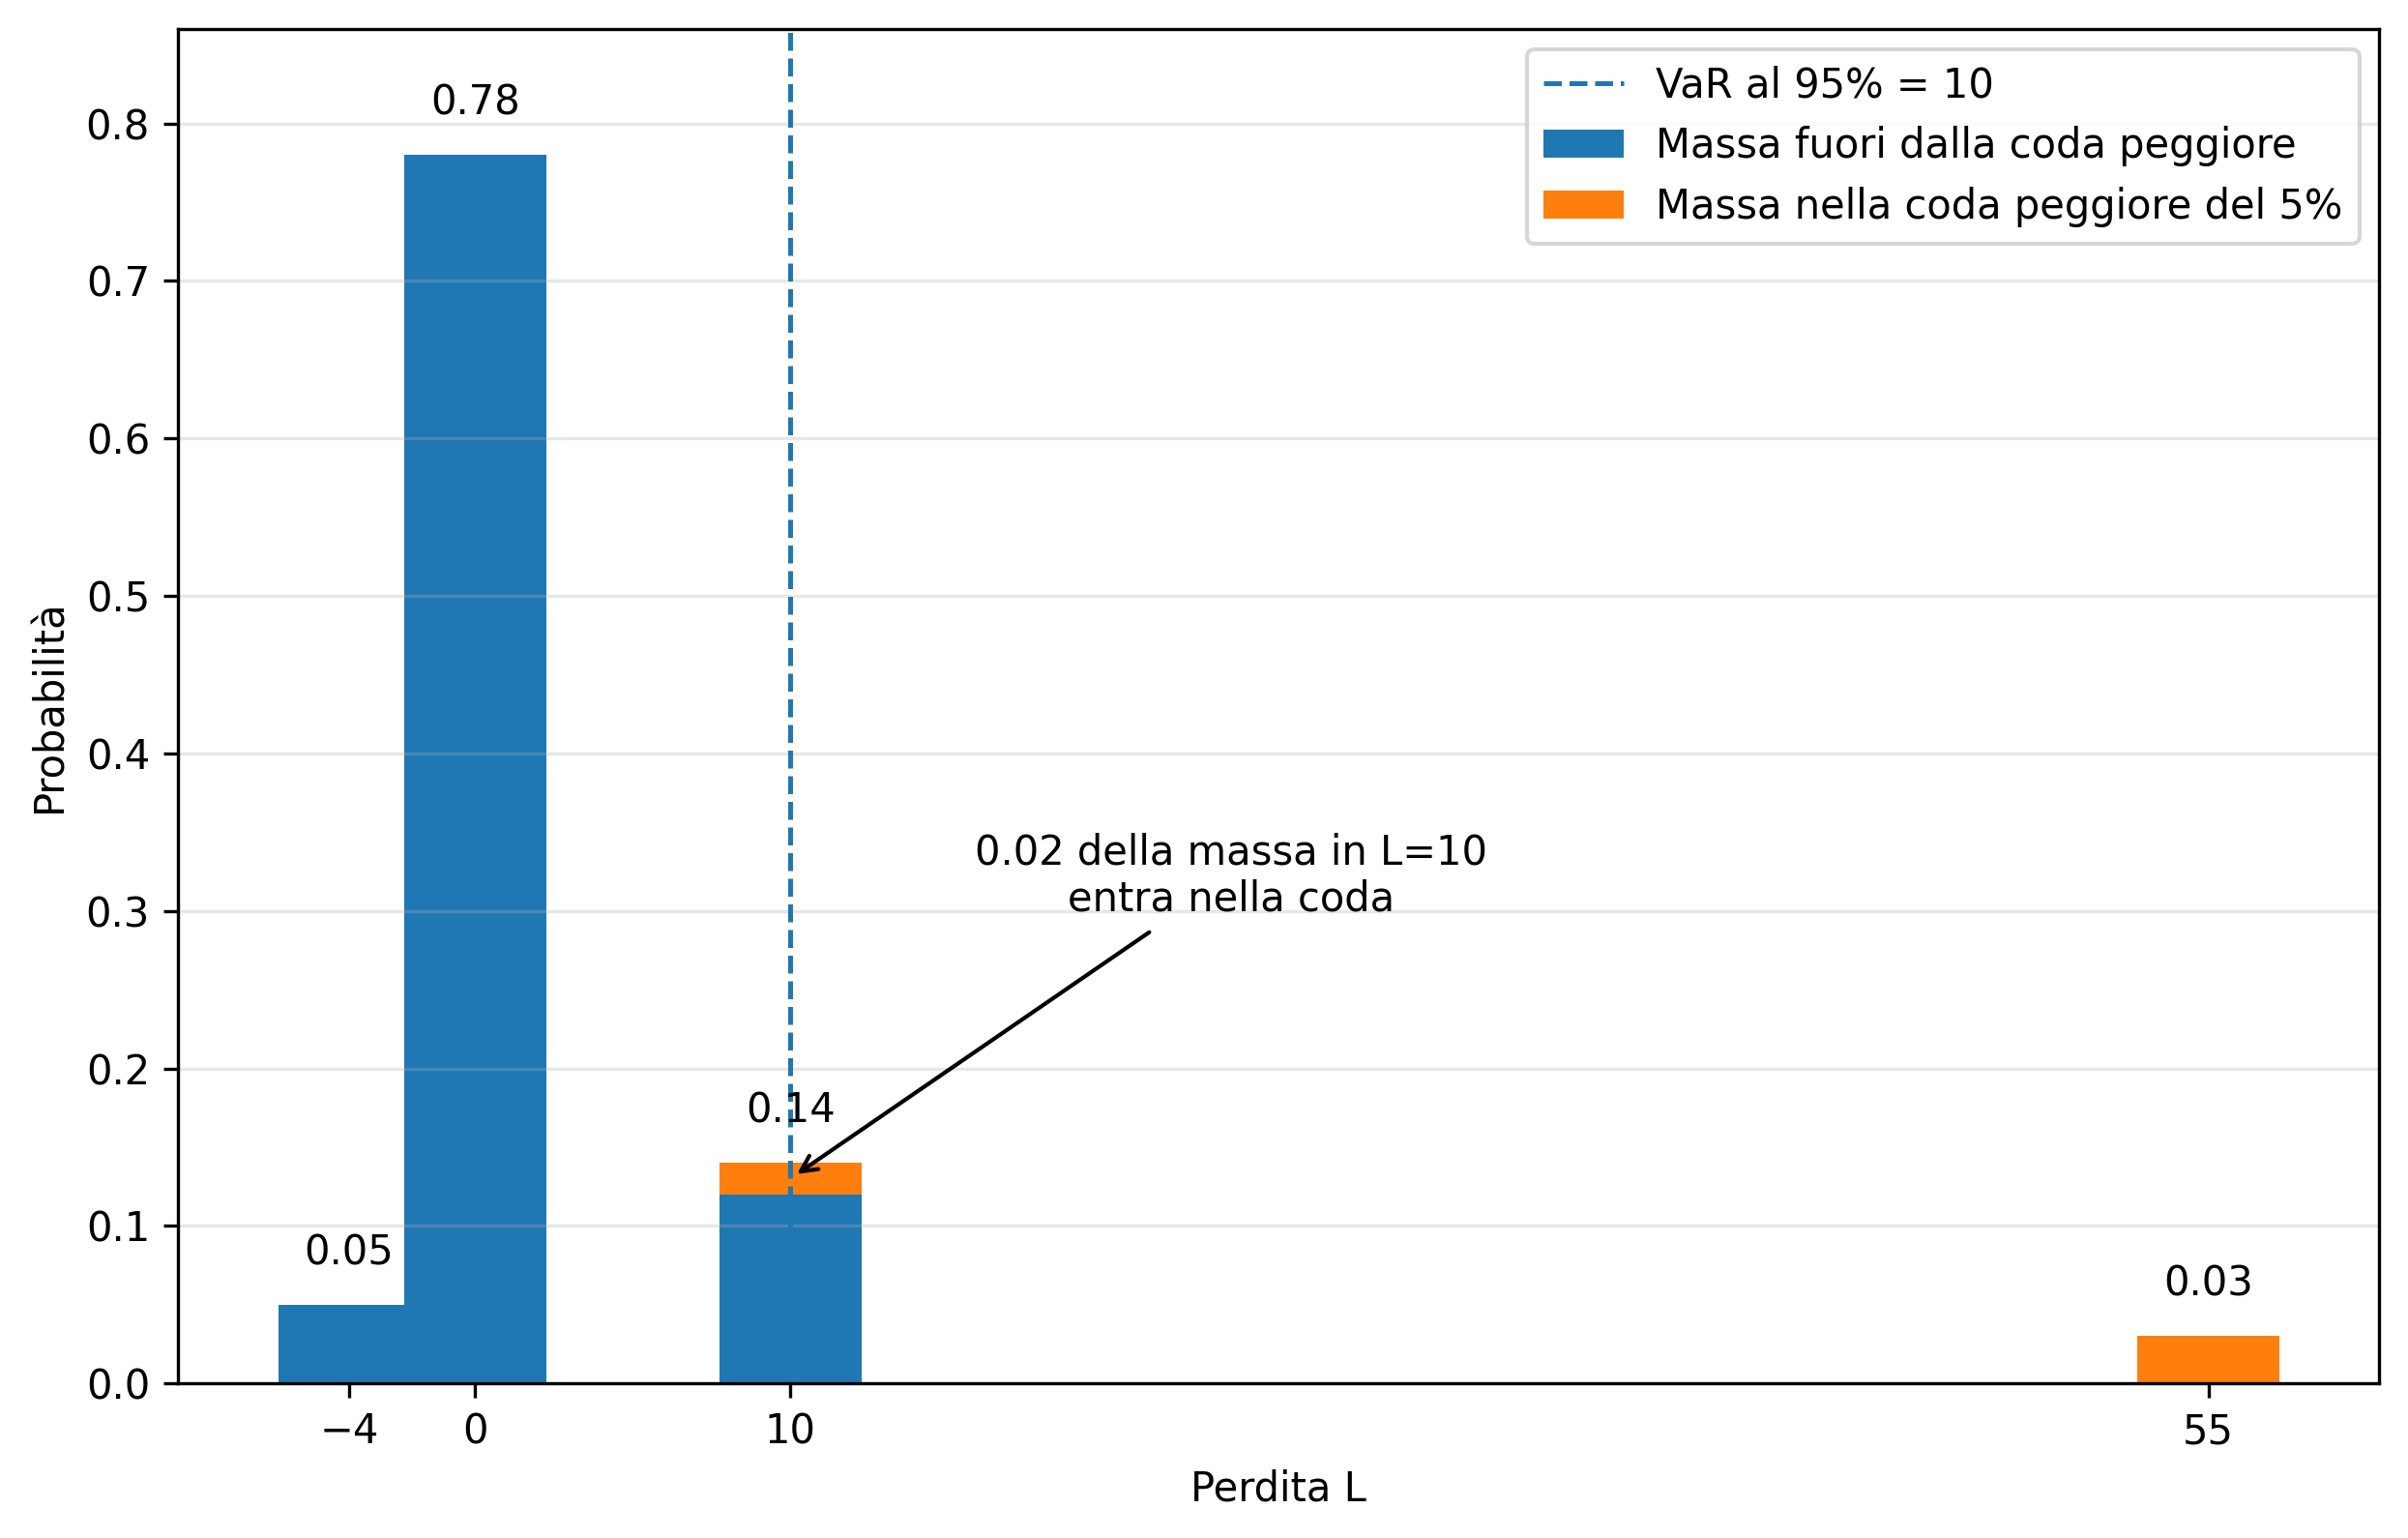
\includegraphics[height=3.9cm]{../graphics/Cap09_CVaR_massa_quantile_esercizio.png}
\end{center}

\begin{center}
{\small Errore da evitare: $\E[L_1\mid L_1\geq 8]\approx 17.18\neq
39.2$, perch\'{e} include \emph{tutta} la massa in $8$. In generale
$\CVaR_{\alpha}(L)\neq\E[L\mid L\geq\VaR_{\alpha}(L)]$ in presenza di
massa nel punto di VaR.}
\end{center}

%TCIMACRO{\TeXButton{Transition: Box Out}{\transboxout}}%
%BeginExpansion
\transboxout%
%EndExpansion
%TCIMACRO{\TeXButton{EndFrame}{\end{frame}}}%
%BeginExpansion
\end{frame}%
%EndExpansion

%***********************************************************
\subsection{VaR e CVaR a confronto}

%TCIMACRO{\TeXButton{BeginFrame}{\begin{frame}}}%
%BeginExpansion
\begin{frame}%
%EndExpansion

\QTR{frametitle}{VaR e CVaR a confronto}

%TCIMACRO{\TeXButton{Transparency}{\setbeamercovered{transparent=20}}}%
%BeginExpansion
\setbeamercovered{transparent=20}%
%EndExpansion

Chiudiamo l'Esercizio B con la misura che ora possediamo:
\[
\begin{array}{lcc}
\hline
& L_A & L_B\\
\hline
\VaR_{0.95} & 10 & 10\\
\CVaR_{0.95} & 36 & 84\\
\hline
\end{array}
\]

\medskip

\begin{stepitemize}
\item Il CVaR distingue ci\`{o} che il VaR dichiarava equivalente: la
probabilit\`{a} della perdita estrema $100$ \`{e} $0.01$ contro
$0.04$.

\item Sul caso guida: $\VaR_{0.95,2}(1)=8$, $\CVaR_{0.95,2}(1)=39.2$
--- la soglia \`{e} modesta, la coda \`{e} severa. I due numeri
raccontano aspetti diversi della stessa distribuzione.

\item Il CVaR \`{e} la misura che ritroveremo nei modelli di
ottimizzazione di portafoglio, nella seconda parte del corso.
\end{stepitemize}

%TCIMACRO{\TeXButton{Transition: Box Out}{\transboxout}}%
%BeginExpansion
\transboxout%
%EndExpansion
%TCIMACRO{\TeXButton{EndFrame}{\end{frame}}}%
%BeginExpansion
\end{frame}%
%EndExpansion

%***********************************************************

%***********************************************************

\section{Il credit default swap}

\subsection{Misurare o prezzare}

%TCIMACRO{\TeXButton{BeginFrame}{\begin{frame}}}%
%BeginExpansion
\begin{frame}%
%EndExpansion

\QTR{frametitle}{Misurare il rischio o prezzare la protezione}

%TCIMACRO{\TeXButton{Transparency}{\setbeamercovered{transparent=20}}}%
%BeginExpansion
\setbeamercovered{transparent=20}%
%EndExpansion

Finora abbiamo \textbf{misurato}: quali perdite possono verificarsi, e
con quali probabilit\`{a}? Ora vogliamo \textbf{prezzare} la
protezione: qual \`{e} oggi il valore di mercato dei flussi futuri?

\medskip

\[
\begin{array}{ccl}
\text{misurazione del rischio}
&
\longrightarrow
&
\text{probabilit\`{a} predittive sotto }\Prob,
\\[2mm]
\text{valutazione di mercato}
&
\longrightarrow
&
\text{valori attesi di flussi attualizzati sotto }\Q.
\end{array}
\]

\medskip

\begin{stepitemize}
\item EL, VaR e CVaR usano la matrice $P^{\Prob}$; il pricing usa la
matrice risk-neutral $P^{\Q}$. Stesso scheletro markoviano, due
domande diverse.

\item Le probabilit\`{a} risk-neutral \textbf{non} rappresentano le
frequenze attese degli eventi: sono pesi che riproducono i prezzi di
mercato.
\end{stepitemize}

%TCIMACRO{\TeXButton{Transition: Box Out}{\transboxout}}%
%BeginExpansion
\transboxout%
%EndExpansion
%TCIMACRO{\TeXButton{EndFrame}{\end{frame}}}%
%BeginExpansion
\end{frame}%
%EndExpansion

%***********************************************************
\subsection{Struttura e gamba di protezione}

%TCIMACRO{\TeXButton{BeginFrame}{\begin{frame}}}%
%BeginExpansion
\begin{frame}%
%EndExpansion

\QTR{frametitle}{Il contratto CDS e la gamba di protezione}

%TCIMACRO{\TeXButton{Transparency}{\setbeamercovered{transparent=20}}}%
%BeginExpansion
\setbeamercovered{transparent=20}%
%EndExpansion

Il \emph{protection buyer} paga un premio periodico $sN$; il
\emph{protection seller} paga $N(1-R)$ al default della
\emph{reference entity}, entro la scadenza $H$. Dal punto di vista del
buyer:
\[
V_{\mathrm{CDS}}(s)
=
\mathrm{PV}_{\mathrm{prot}}
-
\mathrm{PV}_{\mathrm{prem}}(s).
\]

\medskip

\begin{stepitemize}
\item La gamba di protezione paga solo sull'evento $\{\tau_D=h\}$:
\[
\mathrm{PV}_{\mathrm{prot}}
=
N(1-R)
\sum_{h=1}^{H}
d_h\,
\Q(\tau_D=h\mid X_0=i).
\]

\item Le probabilit\`{a} di \textbf{primo ingresso} in default sono le
marginali del Gruppo~2, ora sotto $\Q$:
\[
\Q(\tau_D=h\mid X_0=i)
=
\left[(P^{\Q})^h\right]_{iD}
-
\left[(P^{\Q})^{h-1}\right]_{iD}.
\]
\end{stepitemize}

%TCIMACRO{\TeXButton{Transition: Box Out}{\transboxout}}%
%BeginExpansion
\transboxout%
%EndExpansion
%TCIMACRO{\TeXButton{EndFrame}{\end{frame}}}%
%BeginExpansion
\end{frame}%
%EndExpansion

%***********************************************************
\subsection{Premio equo}

%TCIMACRO{\TeXButton{BeginFrame}{\begin{frame}}}%
%BeginExpansion
\begin{frame}%
%EndExpansion

\QTR{frametitle}{Gamba dei premi e spread equo}

%TCIMACRO{\TeXButton{Transparency}{\setbeamercovered{transparent=20}}}%
%BeginExpansion
\setbeamercovered{transparent=20}%
%EndExpansion

Nel contratto standard i premi sono \textbf{posticipati}: il premio
del periodo $h$ \`{e} pagato in $t=h$, solo se l'emittente \`{e}
ancora in vita ($\{\tau_D>h\}$):
\[
\mathrm{PV}_{\mathrm{prem}}(s)
=
sN
\sum_{h=1}^{H}
d_h\,
\Q(\tau_D>h\mid X_0=i).
\]

Il premio equo $s^{*}$ annulla il valore del contratto,
$\mathrm{PV}_{\mathrm{prem}}(s^{*})=\mathrm{PV}_{\mathrm{prot}}$:
\[
s^{*}
=
(1-R)
\frac{
\displaystyle\sum_{h=1}^{H}d_h\,\Q(\tau_D=h\mid X_0=i)
}{
\displaystyle\sum_{h=1}^{H}d_h\,\Q(\tau_D>h\mid X_0=i)
}.
\]

\medskip

\begin{center}
{\small Marginali al numeratore, sopravvivenze al denominatore: la
struttura temporale del Gruppo~2 \`{e} l'ingrediente di entrambe le
gambe.}
\end{center}

%TCIMACRO{\TeXButton{Transition: Box Out}{\transboxout}}%
%BeginExpansion
\transboxout%
%EndExpansion
%TCIMACRO{\TeXButton{EndFrame}{\end{frame}}}%
%BeginExpansion
\end{frame}%
%EndExpansion

%***********************************************************

%TCIMACRO{\TeXButton{BeginFrame}{\begin{frame}}}%
%BeginExpansion
\begin{frame}%
%EndExpansion

\QTR{frametitle}{Premi posticipati e premi anticipati}

%TCIMACRO{\TeXButton{Transparency}{\setbeamercovered{transparent=20}}}%
%BeginExpansion
\setbeamercovered{transparent=20}%
%EndExpansion

Il premio del periodo $h$ pu\`{o} essere pagato alla fine ($t=h$,
\textbf{posticipato}) oppure all'inizio ($t=h-1$,
\textbf{anticipato}). Sconto e sopravvivenza si valutano alla data di
pagamento:
\[
\mathrm{PV}_{\mathrm{prem}}^{\mathrm{post}}(s)
=
sN\sum_{h=1}^{H}d_{h}\,\Q(\tau_D>h\mid X_0=i),
\]
\[
\mathrm{PV}_{\mathrm{prem}}^{\mathrm{ant}}(s)
=
sN\sum_{h=1}^{H}d_{h-1}\,\Q(\tau_D>h-1\mid X_0=i).
\]

\medskip

\begin{stepitemize}
\item Un pagamento pu\`{o} dipendere solo dall'informazione
disponibile alla data in cui avviene: \`{e} il principio di
adattabilit\`{a} gi\`{a} incontrato nella Lezione~5.

\item Con premi anticipati e $H=1$ l'unico premio cade in $t=0$, dove
$d_0=1$ e $\Q(\tau_D>0)=S(0)=1$. Il coefficiente della gamba dei premi
non sparisce: \textbf{vale} $1$, e
$\mathrm{PV}_{\mathrm{prem}}^\mathrm{ant}(s)=sN$.
\end{stepitemize}

%TCIMACRO{\TeXButton{Transition: Box Out}{\transboxout}}%
%BeginExpansion
\transboxout%
%EndExpansion
%TCIMACRO{\TeXButton{EndFrame}{\end{frame}}}%
%BeginExpansion
\end{frame}%
%EndExpansion




%***********************************************************

%TCIMACRO{\TeXButton{BeginFrame}{\begin{frame}}}%
%BeginExpansion
\begin{frame}%
%EndExpansion

\QTR{frametitle}{Il caso guida sotto la misura di pricing}

%TCIMACRO{\TeXButton{Transparency}{\setbeamercovered{transparent=20}}}%
%BeginExpansion
\setbeamercovered{transparent=20}%
%EndExpansion

Per prezzare il CDS sul caso guida serve la riga risk-neutral dello
stato iniziale. Essa \`{e} \textbf{assegnata}, coerente con i prezzi
di mercato:
\[
\begin{array}{lcccc}
\hline
& \text{upgrade} & \text{invariato} & \text{downgrade} & \text{default}\\
\hline
\text{riga 2 sotto }\Prob & 0.08 & 0.75 & 0.14 & 0.03\\
\text{riga 2 sotto }\Q & 0.075 & 0.745 & 0.145 & 0.035\\
\hline
\end{array}
\]

\begin{stepitemize}
\item La massa si sposta dagli stati favorevoli a downgrade e default:
il mercato, avverso al rischio, prezza la protezione pi\`{u} di quanto
farebbe un investitore neutrale. \`{E} il premio al rischio, letto nei
pesi. Le PD implicite nei CDS superano cos\`{\i} quelle storiche:
$0.035$ contro $0.03$.

\item Premio \textbf{upfront}, gi\`{a} in valore attuale:
$\mathrm{PV}_{\mathrm{prem}}(s)=sN$, senza sconto. La protezione \`{e}
un flusso futuro e incerto, da scontare e ponderare ($R=0.40$,
$d_1=1/1.05$):
\[
\mathrm{PV}_{\mathrm{prot}}
=
100\,(0.60)\,\frac{0.035}{1.05}
=
2,
\qquad
s^{*}
=
\frac{2}{100}
=
200
\text{ punti base}.
\]
\end{stepitemize}

%TCIMACRO{\TeXButton{Transition: Box Out}{\transboxout}}%
%BeginExpansion
\transboxout%
%EndExpansion
%TCIMACRO{\TeXButton{EndFrame}{\end{frame}}}%
%BeginExpansion
\end{frame}%
%EndExpansion

%***********************************************************
\subsection{Spread equo: lettura grafica}

%TCIMACRO{\TeXButton{BeginFrame}{\begin{frame}}}%
%BeginExpansion
\begin{frame}%
%EndExpansion

\QTR{frametitle}{Lo spread equo come punto di equilibrio}

\begin{center}
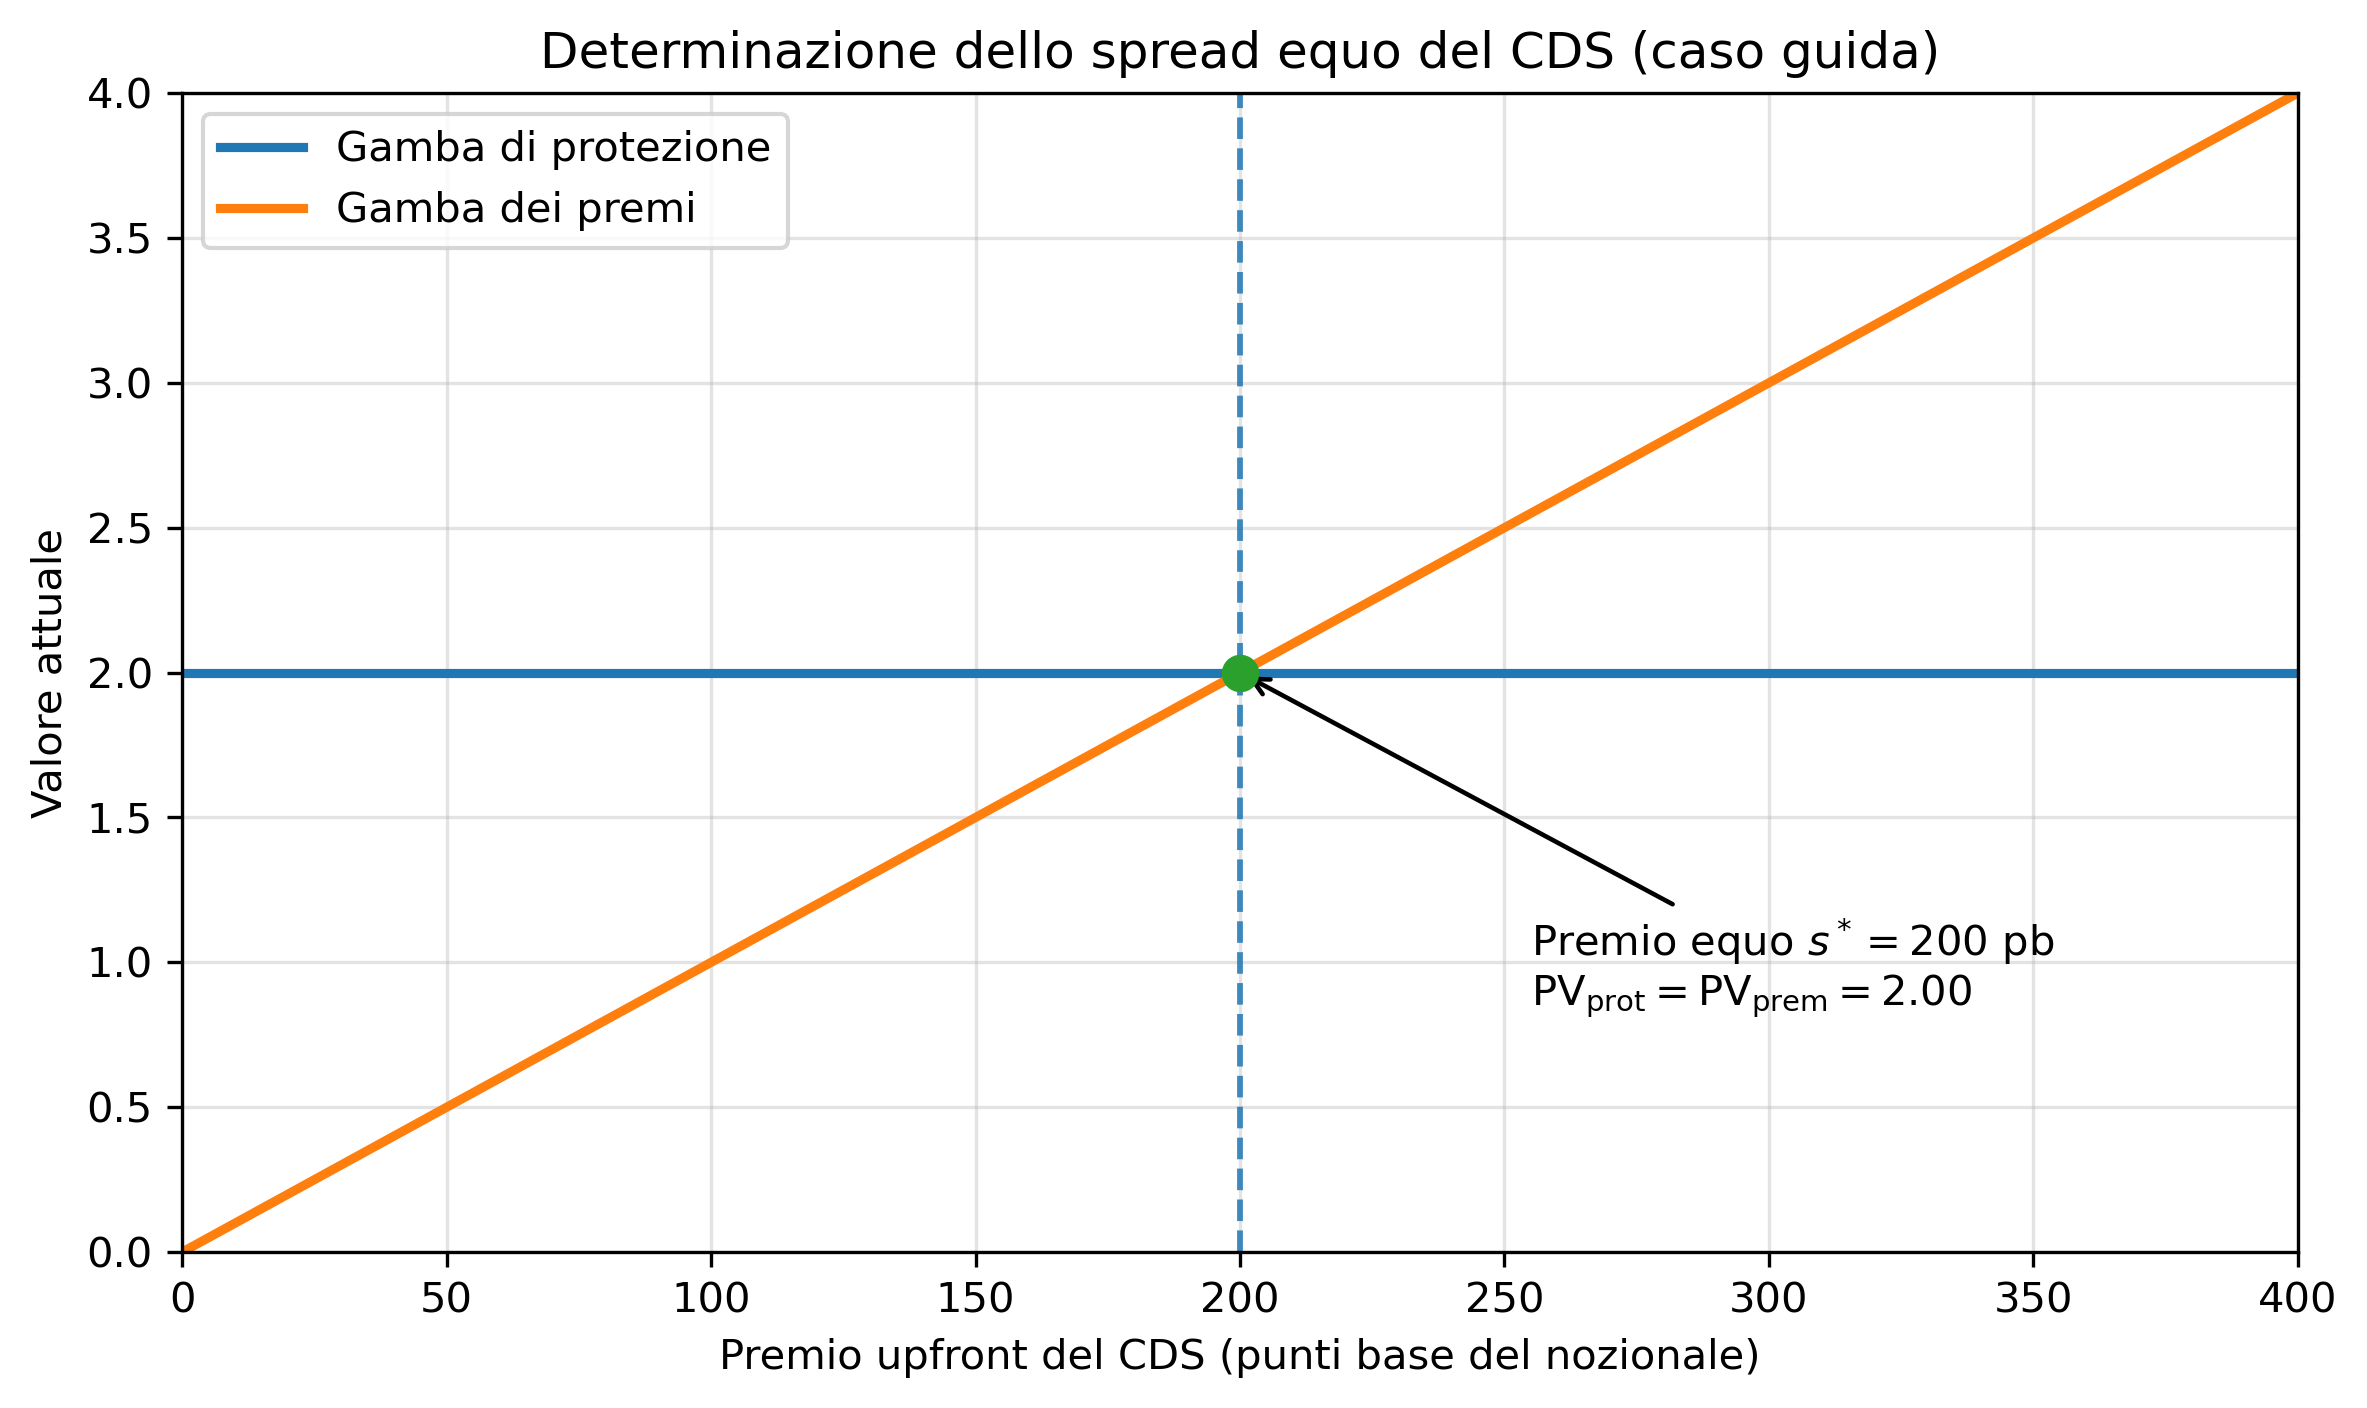
\includegraphics[height=5.6cm]{../graphics/Cap09_CDS_equilibrio_gambe_caso_guida.png}
\end{center}

\medskip

\begin{center}
{\small La gamba di protezione non dipende da $s$: retta orizzontale.
La gamba dei premi cresce linearmente in $s$. 
Lo spread equo $s^{*}$ \`{e} l'ascissa dell'intersezione: per $s<s^{*}$ il contratto ha valore positivo per il \emph{protection buyer}, con $s>s^*$ per il
\emph{seller}.}
\end{center}

%TCIMACRO{\TeXButton{Transition: Box Out}{\transboxout}}%
%BeginExpansion
\transboxout%
%EndExpansion
%TCIMACRO{\TeXButton{EndFrame}{\end{frame}}}%
%BeginExpansion
\end{frame}%
%EndExpansion

%***********************************************************

%***********************************************************

\section{Copertura e rischio residuo}

\subsection{Posizione coperta}

%TCIMACRO{\TeXButton{BeginFrame}{\begin{frame}}}%
%BeginExpansion
\begin{frame}%
%EndExpansion

\QTR{frametitle}{La posizione coperta}

%TCIMACRO{\TeXButton{Transparency}{\setbeamercovered{transparent=20}}}%
%BeginExpansion
\setbeamercovered{transparent=20}%
%EndExpansion

Perdita del protection buyer con copertura:
\[
L^{\mathrm{hedged}}
=
L^{\mathrm{credito}}
-
\Pi^{\mathrm{CDS}}
+
C^{\mathrm{premi}},
\qquad
\Pi^{\mathrm{CDS}}
=
N_{\mathrm{CDS}}(1-R_{\mathrm{CDS}})
\mathbf{1}_{\{\tau_D\leq H\}}.
\]

\begin{center}
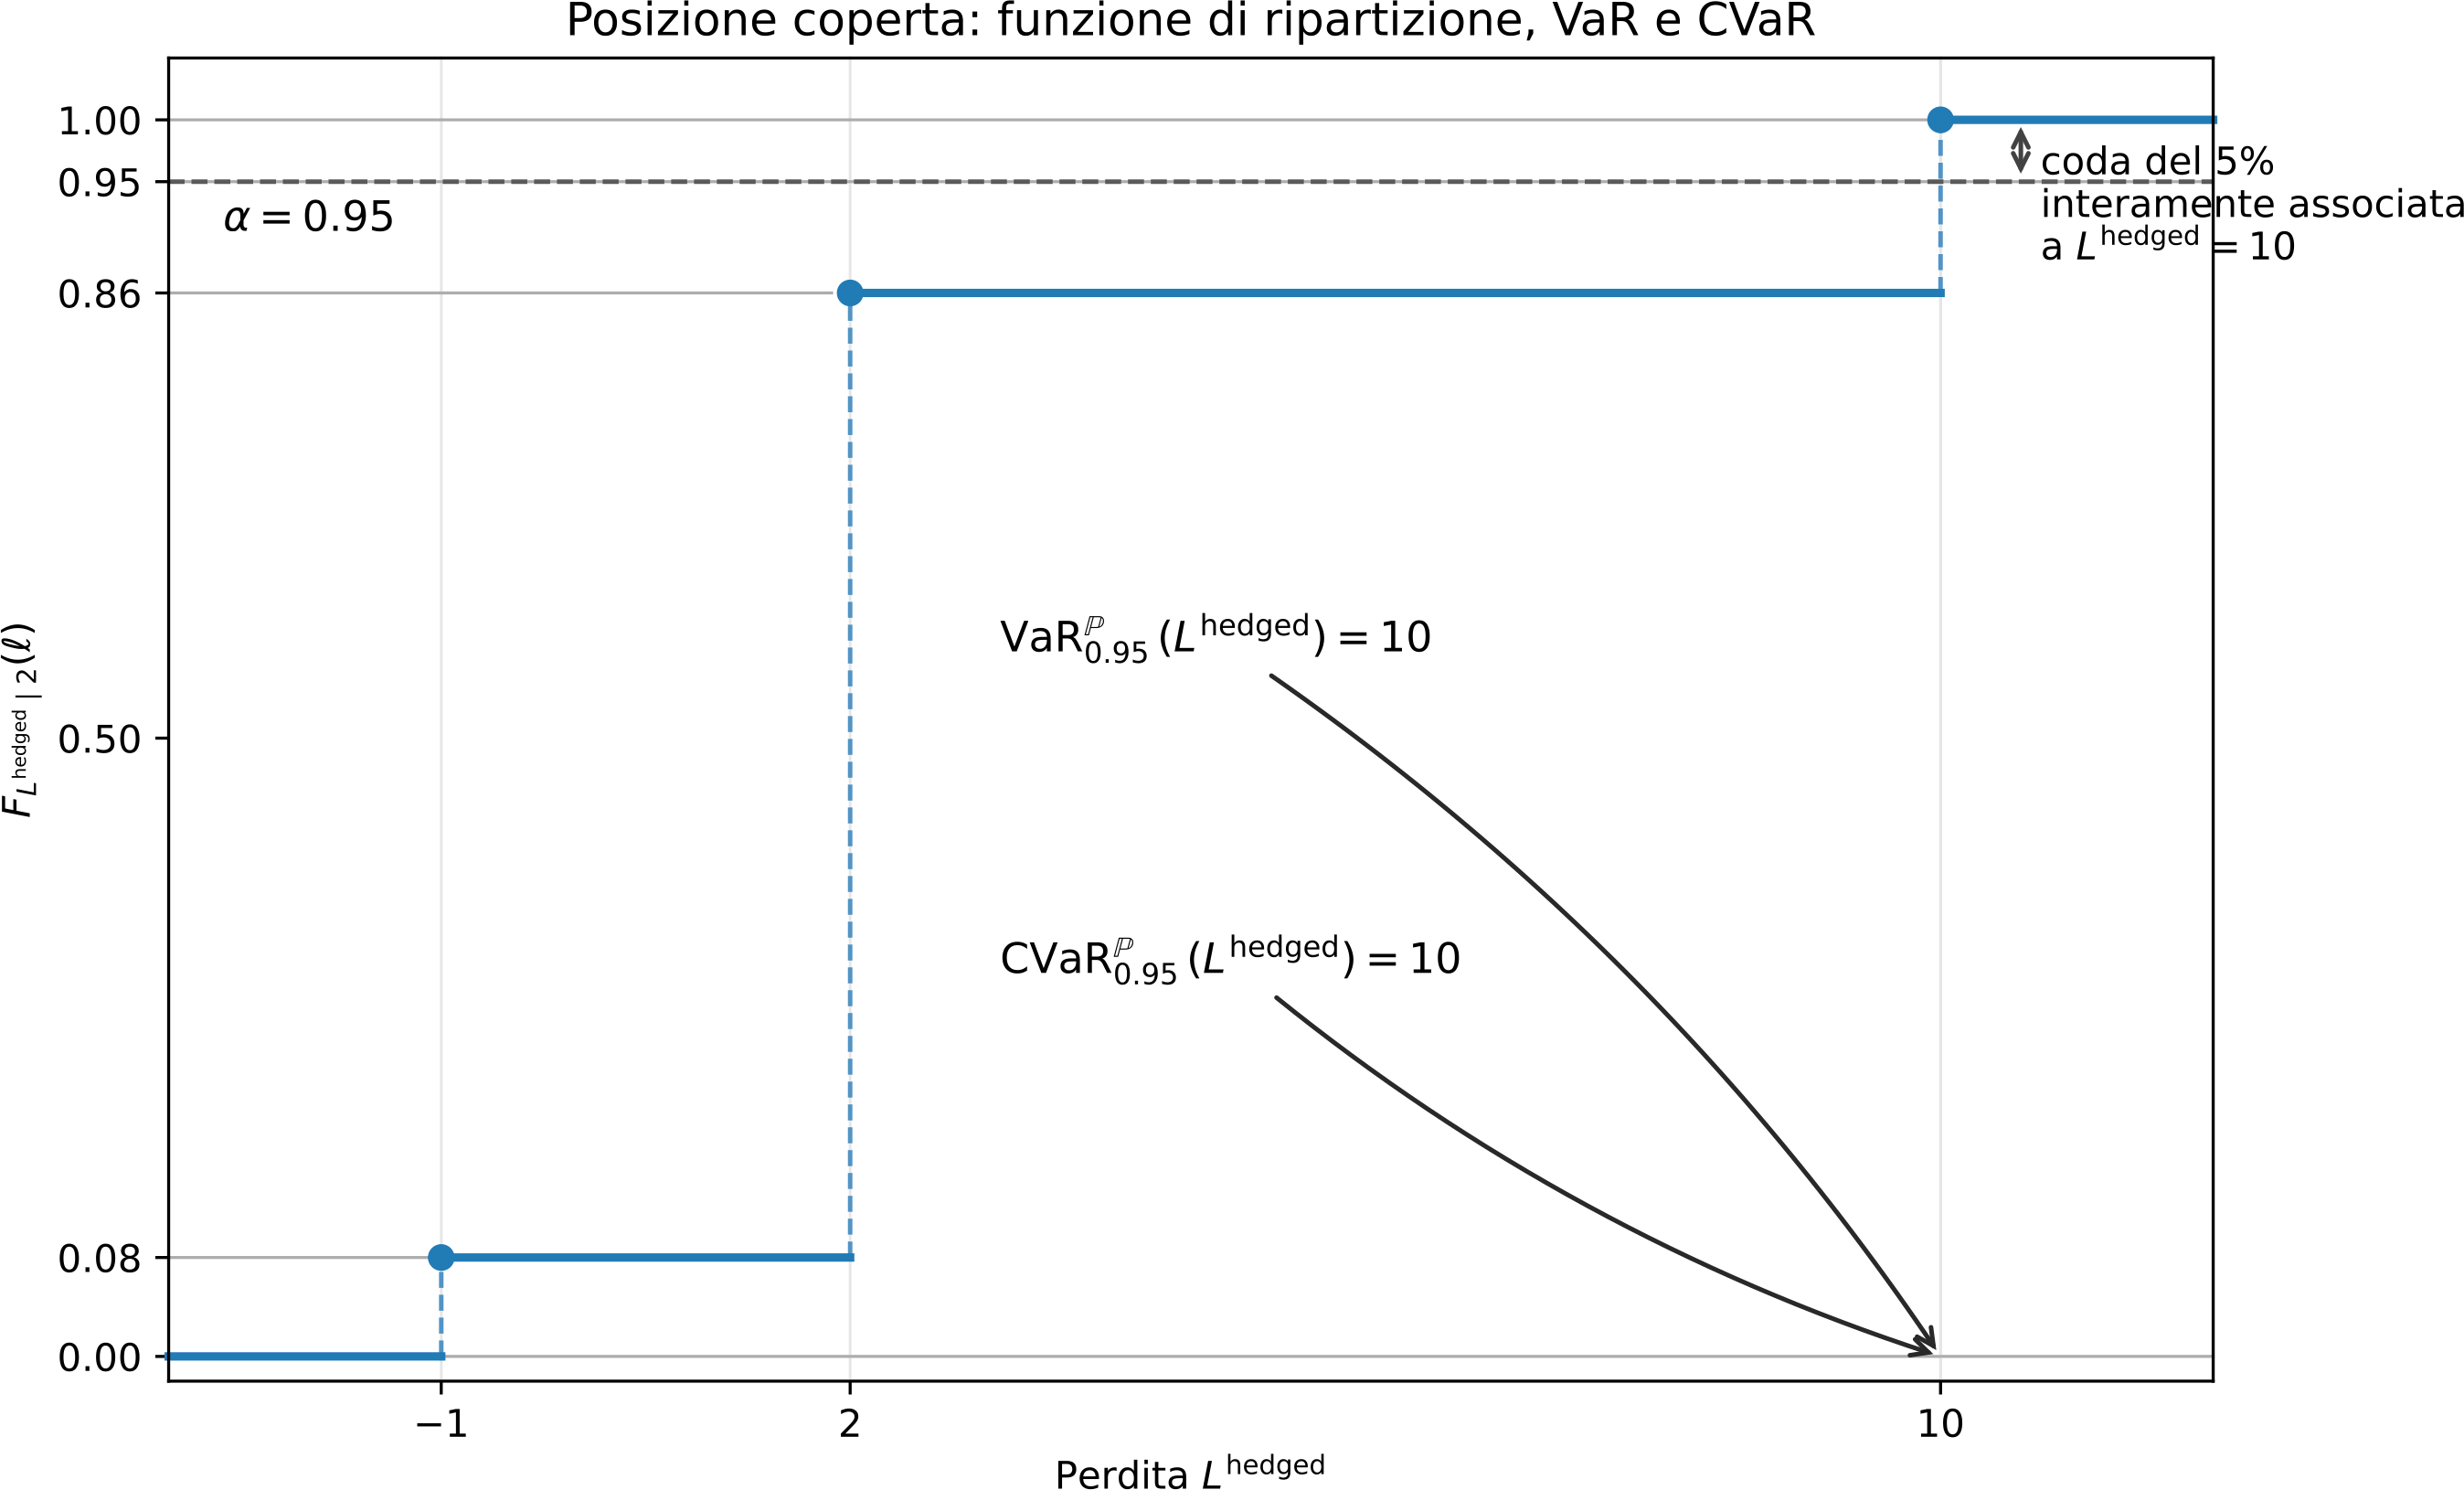
\includegraphics[height=4.5cm]{../graphics/Cap09_cdf_hedged_var_cvar.png}
\end{center}

\begin{center}
{\small Il pagamento di protezione elimina lo scenario estremo: la
coda del $5\%$ \`{e} interamente associata a $L^{\mathrm{hedged}}=10$
e le due misure coincidono, $\VaR_{0.95}=\CVaR_{0.95}=10$. Il costo
dei premi trasla per\`{o} le perdite negli altri stati.}
\end{center}

%TCIMACRO{\TeXButton{Transition: Box Out}{\transboxout}}%
%BeginExpansion
\transboxout%
%EndExpansion
%TCIMACRO{\TeXButton{EndFrame}{\end{frame}}}%
%BeginExpansion
\end{frame}%
%EndExpansion

%***********************************************************
\subsection{Rischio residuo}

%TCIMACRO{\TeXButton{BeginFrame}{\begin{frame}}}%
%BeginExpansion
\begin{frame}%
%EndExpansion

\QTR{frametitle}{Che cosa la copertura non elimina}

%TCIMACRO{\TeXButton{Transparency}{\setbeamercovered{transparent=20}}}%
%BeginExpansion
\setbeamercovered{transparent=20}%
%EndExpansion

\begin{stepitemize}
\item \textbf{Costo dei premi}: la copertura riduce la perdita attesa
sotto $\Prob$ solo se la protezione attesa supera il costo atteso ---
non \`{e} garantito da un premio equo sotto $\Q$.

\item \textbf{Perdite da migrazione}: il CDS default-only non paga per
un semplice downgrade; la perdita mark-to-market resta scoperta.

\item \textbf{Basis risk e mismatch}: nozionale o scadenza del CDS
diversi dall'esposizione lasciano quote di rischio scoperte o
sovracoperte.

\item \textbf{Rischio di controparte}: la protezione vale solo se il
seller paga --- e pu\`{o} deteriorarsi proprio negli scenari in cui
serve.

\item \textbf{Evento economico $\neq$ evento contrattuale}: il
pagamento dipende dalla definizione giuridica del credit event, non
dalla perdita economica subita.
\end{stepitemize}

\medskip

\begin{center}
{\small La qualit\`{a} della copertura si giudica confrontando le
distribuzioni complete di $L^{\mathrm{unhedged}}$ e
$L^{\mathrm{hedged}}$: una riduzione del CVaR non implica una
riduzione di EL o VaR.}
\end{center}

%TCIMACRO{\TeXButton{Transition: Box Out}{\transboxout}}%
%BeginExpansion
\transboxout%
%EndExpansion
%TCIMACRO{\TeXButton{EndFrame}{\end{frame}}}%
%BeginExpansion
\end{frame}%
%EndExpansion

%***********************************************************

%***********************************************************

\section{Sintesi e raccordo}

\subsection{Sintesi della lezione}

%TCIMACRO{\TeXButton{BeginFrame}{\begin{frame}}}%
%BeginExpansion
\begin{frame}%
%EndExpansion

\QTR{frametitle}{Sintesi e raccordo con la Lezione 10}

%TCIMACRO{\TeXButton{Transparency}{\setbeamercovered{transparent=20}}}%
%BeginExpansion
\setbeamercovered{transparent=20}%
%EndExpansion

La catena costruita oggi:
\[
\boxed{
\begin{array}{l}
\text{PD cum./marg./sopravv.}
\;\rightarrow\;
L_h=\ell(X_h,h)
\;\rightarrow\;
\mathrm{EL},\ \VaR,\ \CVaR
\\[1mm]
\qquad\qquad
\rightarrow\;
\text{CDS e copertura}
\quad
{\scriptstyle (P^{\Prob}\ \text{rischio},\ P^{\Q}\ \text{pricing})}
\end{array}
}
\]

\medskip

\begin{stepitemize}
\item Per un \textbf{portafoglio}, la perdita aggregata
$L_h^{\mathrm{port}}=\sum_{n=1}^{N}L_{n,h}$ dipende anche dalla
probabilit\`{a} che downgrade e default si verifichino
\emph{congiuntamente}: \`{e} la dipendenza a governare le code.

\item Con molte esposizioni la distribuzione congiunta non \`{e}
trattabile analiticamente: serve la \textbf{simulazione}. In ciascuna
replica: fattori comuni $\rightarrow$ transizioni individuali
$\rightarrow$ perdite per stato e aggregazione $\rightarrow$ stima
empirica di EL, VaR e CVaR.
\end{stepitemize}


%TCIMACRO{\TeXButton{Transition: Box Out}{\transboxout}}%
%BeginExpansion
\transboxout%
%EndExpansion
%TCIMACRO{\TeXButton{EndFrame}{\end{frame}}}%
%BeginExpansion
\end{frame}%
%EndExpansion

%***********************************************************

\section{Back-up}

\subsection{Separatore}

%TCIMACRO{\TeXButton{BeginFrame}{\begin{frame}}}%
%BeginExpansion
\begin{frame}%
%EndExpansion

\vfill
\begin{center}
{\Huge\bfseries Back-up}
\end{center}
\vfill

%TCIMACRO{\TeXButton{Transition: Box Out}{\transboxout}}%
%BeginExpansion
\transboxout%
%EndExpansion
%TCIMACRO{\TeXButton{EndFrame}{\end{frame}}}%
%BeginExpansion
\end{frame}%
%EndExpansion

%***********************************************************
\subsection{Back-up: probabilit\`{a} condizionata di default}

%TCIMACRO{\TeXButton{BeginFrame}{\begin{frame}}}%
%BeginExpansion
\begin{frame}%
%EndExpansion

\QTR{frametitle}{Back-up: probabilit\`{a} condizionata di default}

%TCIMACRO{\TeXButton{Transparency}{\setbeamercovered{transparent=20}}}%
%BeginExpansion
\setbeamercovered{transparent=20}%
%EndExpansion

Probabilit\`{a} $q_i(h)$ di default nel periodo $h$, \emph{dato} che l'emittente \`{e} sopravvissuto fino a $h-1$ è uguale a:
\[
\Prob(\tau_D=h\mid\tau_D>h-1,\,X_0=i)
=
\frac{\mathrm{PD}_{i}^{\mathrm{marg}}(h)}{S_i(h-1)}
=
\frac{(P^h)_{iD}-(P^{h-1})_{iD}}{1-(P^{h-1})_{iD}}.
\]

\medskip

\begin{stepitemize}
\item In generale $q_i(h)\neq p_{iD}$: per $h>1$ l'emittente pu\`{o}
avere attraversato classi diverse prima dell'inizio del periodo $h$.

\item Scomposizione sui percorsi:
\[
\mathrm{PD}_{i}^{\mathrm{marg}}(h)
=
\sum_{j\neq D}
(P^{h-1})_{ij}\,p_{jD}:
\]
sopravvivere fino a $h-1$ nello stato $j$, poi transitare in $D$.

\item \`{E} l'analogo creditizio del tasso di mortalit\`{a}
attuariale: rischio del periodo, tra i sopravvissuti.
\end{stepitemize}

%TCIMACRO{\TeXButton{Transition: Box Out}{\transboxout}}%
%BeginExpansion
\transboxout%
%EndExpansion
%TCIMACRO{\TeXButton{EndFrame}{\end{frame}}}%
%BeginExpansion
\end{frame}%
%EndExpansion

%***********************************************************
\subsection{Back-up: capitale economico}

%TCIMACRO{\TeXButton{BeginFrame}{\begin{frame}}}%
%BeginExpansion
\begin{frame}%
%EndExpansion

\QTR{frametitle}{Back-up: Credit VaR e capitale economico}

%TCIMACRO{\TeXButton{Transparency}{\setbeamercovered{transparent=20}}}%
%BeginExpansion
\setbeamercovered{transparent=20}%
%EndExpansion

Convenzione del corso: $\mathrm{CreditVaR}_{\alpha,i}(h)
=\VaR_{\alpha,i}(h)$, il quantile della perdita totale. Il
\textbf{capitale economico} \`{e} l'eccesso del quantile sulla media:
\[
\mathrm{EC}_{\alpha,i}(h)
=
\VaR_{\alpha,i}(h)
-
\mathrm{EL}_i(h).
\]

\medskip

\begin{stepitemize}
\item Tre grandezze distinte: $\VaR$ \`{e} la perdita al quantile
$\alpha$; $\mathrm{EL}$ la perdita media; $\mathrm{EC}$ la perdita
corrispondente al quantile $\alpha$ \emph{eccedente} la media.

\item Sul caso guida:
\[
\mathrm{EC}_{0.95,2}(1)
=
8-2.68
=
5.32.
\]

\item Logica gestionale: la EL \`{e} un costo, coperto dagli
accantonamenti; l'EC \`{e} rischio, coperto dal capitale. Ritorner\`{a}
nella Lezione~10 sul portafoglio.
\end{stepitemize}

%TCIMACRO{\TeXButton{Transition: Box Out}{\transboxout}}%
%BeginExpansion
\transboxout%
%EndExpansion
%TCIMACRO{\TeXButton{EndFrame}{\end{frame}}}%
%BeginExpansion
\end{frame}%
%EndExpansion

%***********************************************************
\subsection{Back-up: rappresentazione di ottimizzazione del CVaR}

%TCIMACRO{\TeXButton{BeginFrame}{\begin{frame}}}%
%BeginExpansion
\begin{frame}%
%EndExpansion

\QTR{frametitle}{Back-up: il CVaR come problema di minimo}

%TCIMACRO{\TeXButton{Transparency}{\setbeamercovered{transparent=20}}}%
%BeginExpansion
\setbeamercovered{transparent=20}%
%EndExpansion

Il CVaR ammette la rappresentazione
\[
\CVaR_{\alpha}(L)
=
\min_{\eta\in\R}
\left\{
\eta
+
\frac{1}{1-\alpha}
\E\left[(L-\eta)^{+}\right]
\right\},
\qquad
(x)^{+}=\max\{x,0\}.
\]

\medskip

\begin{stepitemize}
\item $(L-\eta)^{+}$ conta solo gli \textbf{eccessi} oltre la soglia
$\eta$; la funzione da minimizzare \`{e} convessa e un minimizzatore
pu\`{o} essere scelto tra i quantili di livello $\alpha$.

\item Verifica sul caso guida, $\eta=8$:
\[
8+\frac{1}{0.05}\,\E\left[(L_1-8)^{+}\right]
=
8+\frac{(60-8)(0.03)}{0.05}
=
8+31.2
=
39.2.
\]
Lo stesso valore ottenuto in lezione con il calcolo della coda.

\item \`{E} la forma con cui il CVaR entrer\`{a} nei problemi di
ottimizzazione di portafoglio (Lezioni~12--16): soglia $\eta$ e
eccessi diventano variabili e vincoli lineari.
\end{stepitemize}

%TCIMACRO{\TeXButton{Transition: Box Out}{\transboxout}}%
%BeginExpansion
\transboxout%
%EndExpansion
%TCIMACRO{\TeXButton{EndFrame}{\end{frame}}}%
%BeginExpansion
\end{frame}%
%EndExpansion

%***********************************************************
\subsection{Back-up: la matrice risk-neutral}

%TCIMACRO{\TeXButton{BeginFrame}{\begin{frame}}}%
%BeginExpansion
\begin{frame}%
%EndExpansion

\QTR{frametitle}{Back-up: la matrice $P^{\Q}$ e il pricing}

%TCIMACRO{\TeXButton{Transparency}{\setbeamercovered{transparent=20}}}%
%BeginExpansion
\setbeamercovered{transparent=20}%
%EndExpansion

$P^{\Q}=(p_{ij}^{\Q})$ con $p_{ij}^{\Q}=\Q(X_{t+1}=j\mid X_t=i)$;
per una catena omogenea sotto $\Q$,
$\Q(X_h=j\mid X_0=i)=[(P^{\Q})^h]_{ij}$.

\medskip

Se il flusso alla data $t$ dipende solo dallo stato, $C_t=c_t(X_t)$, e
lo sconto $D(0,t)$ \`{e} deterministico:
\[
V_0
=
\E_{\Q}\left[\sum_{t=1}^{T}D(0,t)\,C_t\right]
=
\sum_{t=1}^{T}
D(0,t)
\sum_{j\in\mathcal{I}}
c_t(j)
\left[\left(P^{\Q}\right)^t\right]_{ij}.
\]

\medskip

\begin{stepitemize}
\item La struttura del pricing: $P^{\Q}\rightarrow$ probabilit\`{a}
risk-neutral dei flussi $\rightarrow$ valore atteso attualizzato
$\rightarrow$ valore di mercato.

\item In generale $P^{\Prob}\neq P^{\Q}$: le probabilit\`{a} fisiche
riflettono la dinamica predittiva; quelle risk-neutral incorporano
anche la remunerazione richiesta per l'esposizione al rischio.
\end{stepitemize}

%TCIMACRO{\TeXButton{Transition: Box Out}{\transboxout}}%
%BeginExpansion
\transboxout%
%EndExpansion
%TCIMACRO{\TeXButton{EndFrame}{\end{frame}}}%
%BeginExpansion
\end{frame}%
%EndExpansion

%***********************************************************


%TCIMACRO{\TeXButton{BeginFrame}{\begin{frame}}}%
%BeginExpansion
\begin{frame}%
%EndExpansion

\QTR{frametitle}{Come si pagano i premi nella pratica}

%TCIMACRO{\TeXButton{Transparency}{\setbeamercovered{transparent=20}}}%
%BeginExpansion
\setbeamercovered{transparent=20}%
%EndExpansion

\begin{stepitemize}
\item \textbf{Standard di mercato}: premi trimestrali posticipati,
alle date convenzionali del 20 marzo, giugno, settembre e dicembre.
Al default \`{e} dovuto il rateo maturato dall'ultimo pagamento:
conferma che la copertura viene pagata \emph{dopo} averne goduto.

\item \textbf{Dal 2009} (riforma dei contratti standard): la cedola
corrente \`{e} fissata a valori convenzionali e la differenza rispetto
al premio equo \`{e} regolata con un pagamento \textbf{upfront} alla
stipula, positivo o negativo.

\item \textbf{Nel nostro caso a un periodo} adottiamo la forma pi\`{u}
semplice: premio interamente upfront, versato in $t=0$. Pagamento
certo e immediato:
\[
d_0=1,
\qquad
\Q(\tau_D>0)=S(0)=1
\quad\Longrightarrow\quad
\mathrm{PV}_{\mathrm{prem}}(s)=sN.
\]
Il coefficiente della gamba dei premi non sparisce: \textbf{vale} $1$.
\end{stepitemize}

\medskip

\begin{center}
{\small Un pagamento pu\`{o} dipendere solo dall'informazione
disponibile alla data in cui avviene: \`{e} il principio di
adattabilit\`{a} della Lezione~5.}
\end{center}

%TCIMACRO{\TeXButton{Transition: Box Out}{\transboxout}}%
%BeginExpansion
\transboxout%
%EndExpansion
%TCIMACRO{\TeXButton{EndFrame}{\end{frame}}}%
%BeginExpansion
\end{frame}%
%EndExpansion




\end{document}